\documentclass[a4paper,12pt]{article}
\usepackage{fixltx2e}
\usepackage{amssymb}
\usepackage{hyperref}
\usepackage{pdfpages}
\usepackage{caption}
\usepackage{subcaption}
\begin{document}
\title{Mesoscopic Modelling of Burst Suppression Under Anaesthesia}
\author{Matthew Walsh\\
   \small Brain and Psychological Sciences Research Centre (BPsyC),\\
   \small Swinburne University of Technology, Hawthorn, Victoria 3122, Australia; \\
   \texttt{matthew.walsh@gmail.com}\\
  \and
    David Liley\\
   \small  Brain and Psychological Sciences Research Centre (BPsyC),\\
   \small Swinburne University of Technology, Hawthorn, Victoria 3122, Australia; \\
   \small Cortical Dynamics Ltd, Hawthorn. Victoria 3122, Australia\\
   \texttt{dliley@swin.edu.au}}
\maketitle

\begin{abstract}
The burst suppression pattern is well recognized as
a major class of generalised electroencephlagram (EEG) waveform abnormality 
and is evoked by a variety of anesthetic agents. 
While the electroencephalographic phenomenon and clinical
implications of burst suppression have been studied extensively, the physiological mechanisms
underlying its emergence remain unresolved and obscure. 

While the model of Liley et. al. has been shown to account for many of the major features of the 
mammalian electroencephlagram, because of a strong coupling between excitatory and inhibitory population dynamics,  
it is unlikely to display burst suppression. This is because of the inability of simulated anesthetic action 
to induce the dynamics on multiple timescales that underlie bursting.
However the addition of a mean field driven slow wave system to the Liley model introduces 
multiple timescale behavior to the Liley model.

The extended Liley model is shown to exhibit burst suppression under physiologically 
plausible parameterisations for anesthesia with a wide variety of bursting behavior. 
This paper provides an overview of such dynamics and their relevance for a more 
complete physiological understanding of the EEG.

\end{abstract}
\section{Introduction}
Prior to the development of the modern intensive care unit in the early
1960s, featuring intubation, artificial respiration and comprehensive
physiological monitoring, reports of the electroencephalographic
pattern of burst suppression were confined to animal studies involving
deep anaesthesia and the odd case of psychosurgery (Niedermeyer,
2009). Since then the burst suppression pattern is now recognized as
a major class of generalised EEG waveform abnormality of diagnostic
and prognostic significance that is encountered in a range of
encephalopathic conditions, in addition to its pharmacological genesis
by a variety of sedative and anaesthetic agents. Typically the burst
suppression pattern consists of bursts of high amplitude slow, sharp or
spiking activity electroencephalographic activity separated by periods
of electroencephalographic suppression (isoelectricity). The oscillatory
features of the bursts, together with their duration and the duration of
suppressed periods show a high degree of variability that reflects its
myriad of initiating causes (see Figure \ref{fig:burst_examples} for examples). First identified
during deep anaesthesia with tribromoethanol in cats (Derbyshire et al,
1936), labelled “burst-suppression pattern” by Swank \& Watson (1948) during barbiturate and ether anaesthesia in dogs,
it is now
associated with cortical deafferentation (Henry \& Scoville, 1952),
cerebral anoxia and hypoxia, various types of intracortical lesions
(Fischer-Williams, 1963), deep coma, various infantile
encephalopathies, the final stages of deteriorated status epilepticus
(Trieman et al 1990), hypothermia, and high levels of many sedative
and anaesthetic agents (Schwartz et al, 1989; Akrawi et al 1996).

Burst suppression in the absence of anaesthesia is in general
associated with a very poor prognosis. Grigg-Damberger et al (1989)
found that the neonatal appearance of burst suppression, even if
transient, was a portent of death or severe neurodevelopmental
disability in 93\% of infants who were followed up subsequent to the
appearance of electroencephalographic evidence of neonatal burst
suppression. In adult populations while an anoxic/hypoxic burst
suppression pattern signals a serious pathophysiological event the
outcome is not necessarily fatal and recovery with or without severe
neurological damage is possible (Niedermeyer, 2009). The results of
experimental work with EEG monitoring in rats reveals that animals with
greater rates of high amplitude bursts had a better survival and
neurological outcome compared to those with lower rates of low
amplitude bursts (Geocadin et al, 2002).

While the electroencephalographic phenomenon and clinical
implications of burst suppression have been studied extensively
(Niedermeyer, 2009; Brenner, 1985) the physiological mechanisms
underlying its emergence remain unresolved and obscure. However the
phenomenal resemblance of the patterns of burst suppression to
disorders of neuronal hyperexcitability suggests that similar
physiological mechanisms may be at root. For example the bursting
during burst suppression is often associated with myoclonic jerks
resembling those seen during epileptic fits. Further, during burst
suppression induced by various halogenated anaesthetic agents, bursts
can be readily evoked by auditory, visual or somatosensory stimuli
(Hartikainen et al, 1995). Like generalised epileptiform activity, bursts
are recorded simultaneously at multiple electrode derivations, implying
the wide synchronisation of neuronal activity. Not surprisingly then, in
clinical practice the boundaries between what constitutes coma
induced burst suppression and what is defined as ictal seizure activity
is blurred (Amzica, 2009; Hirsch et al, 2004). While such
differentiation may be one of only semantics practically speaking there
nevertheless may be important clinical implications if they respond
differentially to pharmacotherapy and have different prognostic
outcomes, thus motivating attempts to better clarify such a
distinction.

Surprisingly many anaesthetic agents, at levels well below that needed
to induce burst suppression, quite commonly induce epileptiform
activity (Voss et al, 2008). While such epileptiform activity rarely
progresses to clinically apparent seizures (Garcia-Morales et al, 2002)
the presence of such activity nevertheless is believed to indicate some
form of incipient cortical hyperexcitability. Indeed a number of
mesoscopic mean field models developed to account for the
electroencephalographic features of anaesthetic action (Bojak \& Liley,
2005; Steyn-Ross et al, 1999), based on parameterising empirically
identified sub-cellular and molecular targets, have been able to account
for the pro-convulsant properties of many anaesthetic agents known
to have seizurogenic potential (Wilson et al, 2006; Liley \& Bojak,
2005). Given that the majority of anaesthetic agents induce burst
suppression it is therefore natural to inquire whether these mesoscopic
mean field models of electrocortical anaesthetic action are able to
account for the appearance of drug-induced burst suppression, and in
doing so shed light on the pathophysiological mechanisms of burst
suppression and epilepsy in general.

\begin{figure}
	\label{fig:burst_examples}
	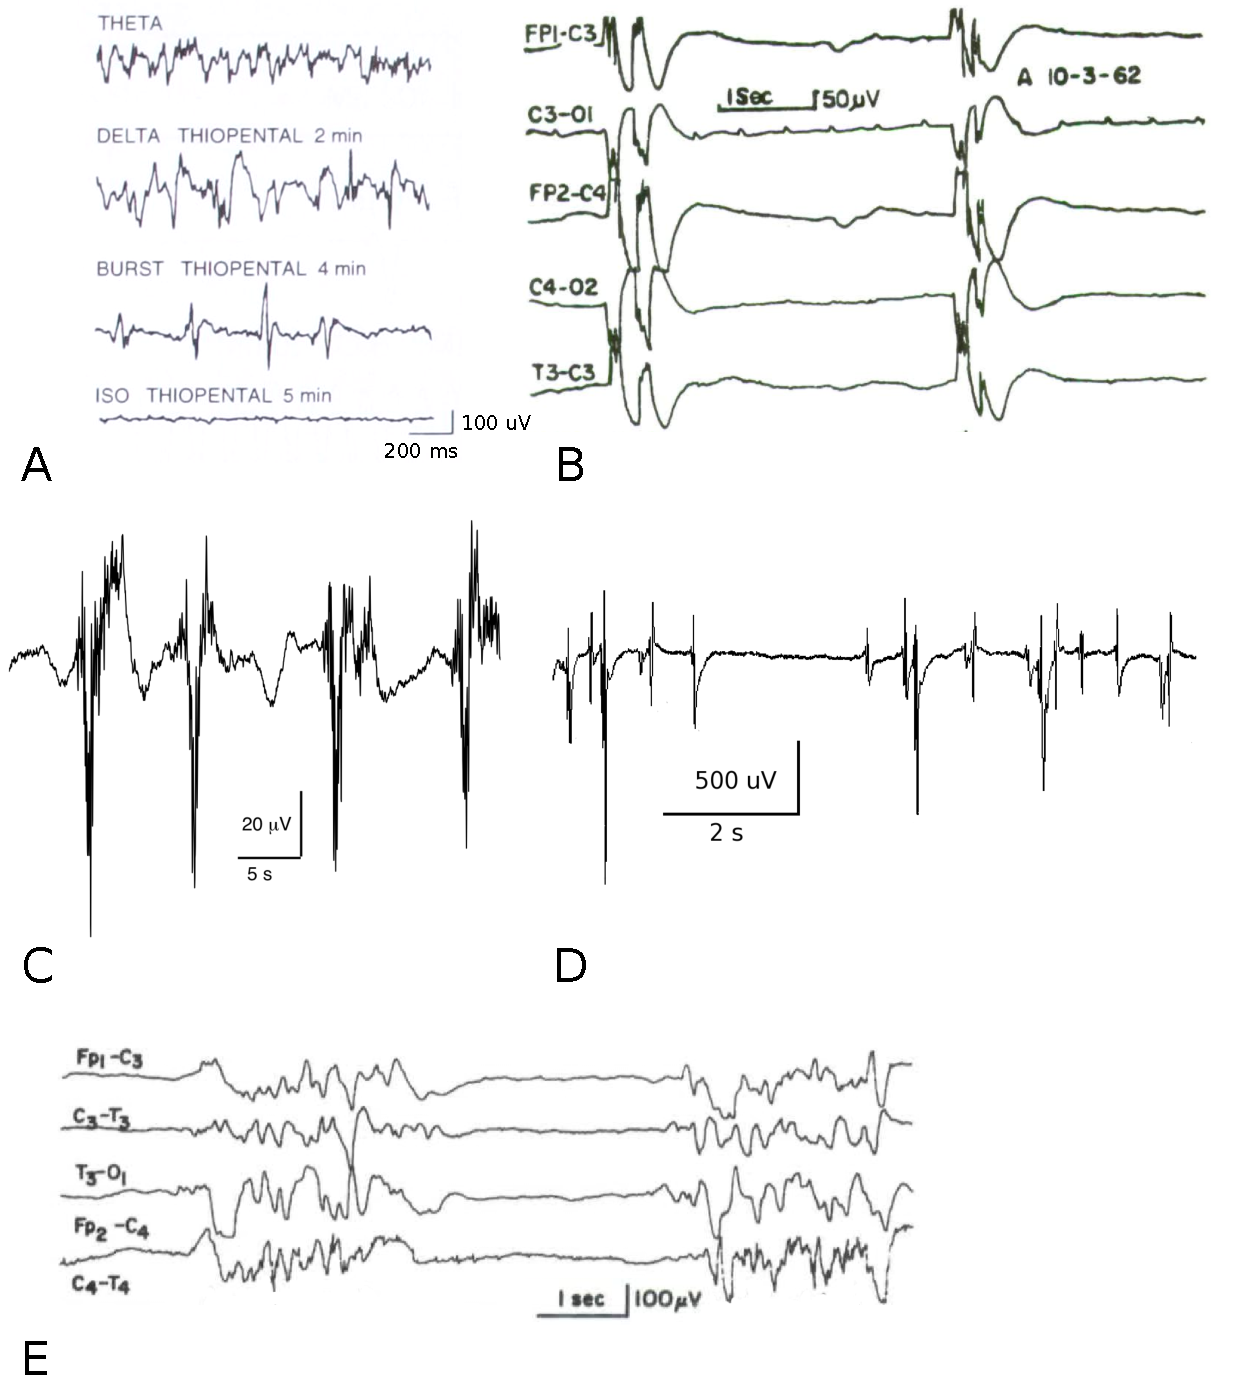
\includegraphics[scale=0.7]{chosen-frontiers-2012/burst_examples.pdf}
	\caption{Example traces of electroencephalogram and
electrocorticogram illustrating the heterogeneity of burst suppression
patterns. (A) changes in neocortical electroencephalogram in the rat,
recorded using dural surface electrodes, in response to a 5 mg/kg/min
thiopental infusion (figure reproduced with permission from Lukatch \&
MacIver, 1996). (B) electroencephalogram recorded in acute anoxia
showing a clear burst suppression pattern with grouped spikes (figure
reproduced with permission from Hockaday et al, 1965). (C) burst
suppression pattern during closed loop target controlled propofol
infusion at a target level of approximately 15 μg/ml (data courtesy of
Professor Michel Struys, Groningen). Note the bursts consist of fast
activity (> 10 Hz) on a slow wave background. (D) electrocorticogram
obtained from an adult merino sheep during deep enflurane anaethesia,
demonstrating high amplitude spikes interspersed with isoelectric
periods of variable length (figure reproduced with permission from
Voss et al, 2006). (E) electroencephalogram recorded from a 3 month
old infant suffering from infantile myoclonic encephalopathy
(reproduced with permission from Niedermeyer, 2005).}
\end{figure}

\section{Methods}
\subsection{Mesoscopic mean field modelling of electrocortical activity}
The electroencephalogram and electrocorticogram arise out of the
cooperative activity of many thousands of neurons. A single
electroencephalographic electrode records the synaptically induced
currents of well over a 100,000 neurons (Nunez \& Srinivasan, 2006)
and thus detailing each neurons contribution to this summed activity
would appear superfluous. For this reason it is preferable instead to
model the activity of populations of neurons. One general way of
achieving this, in which known stochastic fluctuations can be included,
is to dynamically evolve the probability distributions associated with
the states of the neuronal ensemble. While in principle providing a
rigorous way forward the formulation of such stochastic equations of
motion entails a great deal of physiological uncertainty. For this and
other reasons (Deco et al, 2008) a more resolute path is to
dynamically evolve some average quantity such as the mean soma
membrane potential or the mean firing rate of some suitably defined
neuronal ensemble. In this manner a mesoscopic level model can be
developed which acts as a bridge between cellular (or microscopic)
level activity and whole brain (or macroscopic) level behaviour.
While the current mathematical approach for formulating the equations
of motion for the activity of neuronal populations or masses, stems
principally from the works of Wilson \& Cowan (1973, 1972), Nunez
(1974), Freeman (1975) and Amari (1975, 1977), they are not
particularly successful in articulating the genesis of rhythmic activity in
the EEG and its modulation by pharmacological agents, due to a range
of mathematical simplifications that cannot be justified by an appeal to
physiology. For this reason a range of biologically more refined
neuronal populations models have been developed (Deco et al, 2008)
that form a more appropriate basis from which to model the
physiological genesis of the electroencephalogram. The model of Liley
et al (2005; 2003; 2002; 1999) is one such model and will be the
focus of our attempts to account for the phenomenon of burst
suppression.

The model of Liley et al (2011; 2005; 2003; 2002; 1999) is able to
account for the major features of the mammalian
electroencephalogram in the context of a parameterisation that
accords with physiological measurement and experiment. Because it
aims to provide a dynamical description of the electroencephalogram
the model is spatially coarse-grained over the approximate extent of a
cortical macrocolumn, reflecting the general physiological wisdom that
such columniation signifies populations of neurons having similar
functional behaviour and anatomical connectivity. The multiple
interactions between individual neurons are replaced by effective feedforward
and feed-back interactions between the mean activity (or
“mean fields”) of excitatory and inhibitory populations of neurons over
the spatial extent of the column. In this way mammalian neocortex is
conceived as consisting of localized populations of excitatory and
inhibitory neurons interacting by all possible combinations of
feedforward and feedback connectivity interacting globally via long
range excitatory connections (Figure \ref{fig:liley_schema}).

\begin{figure}
\label{fig:liley_schema}
		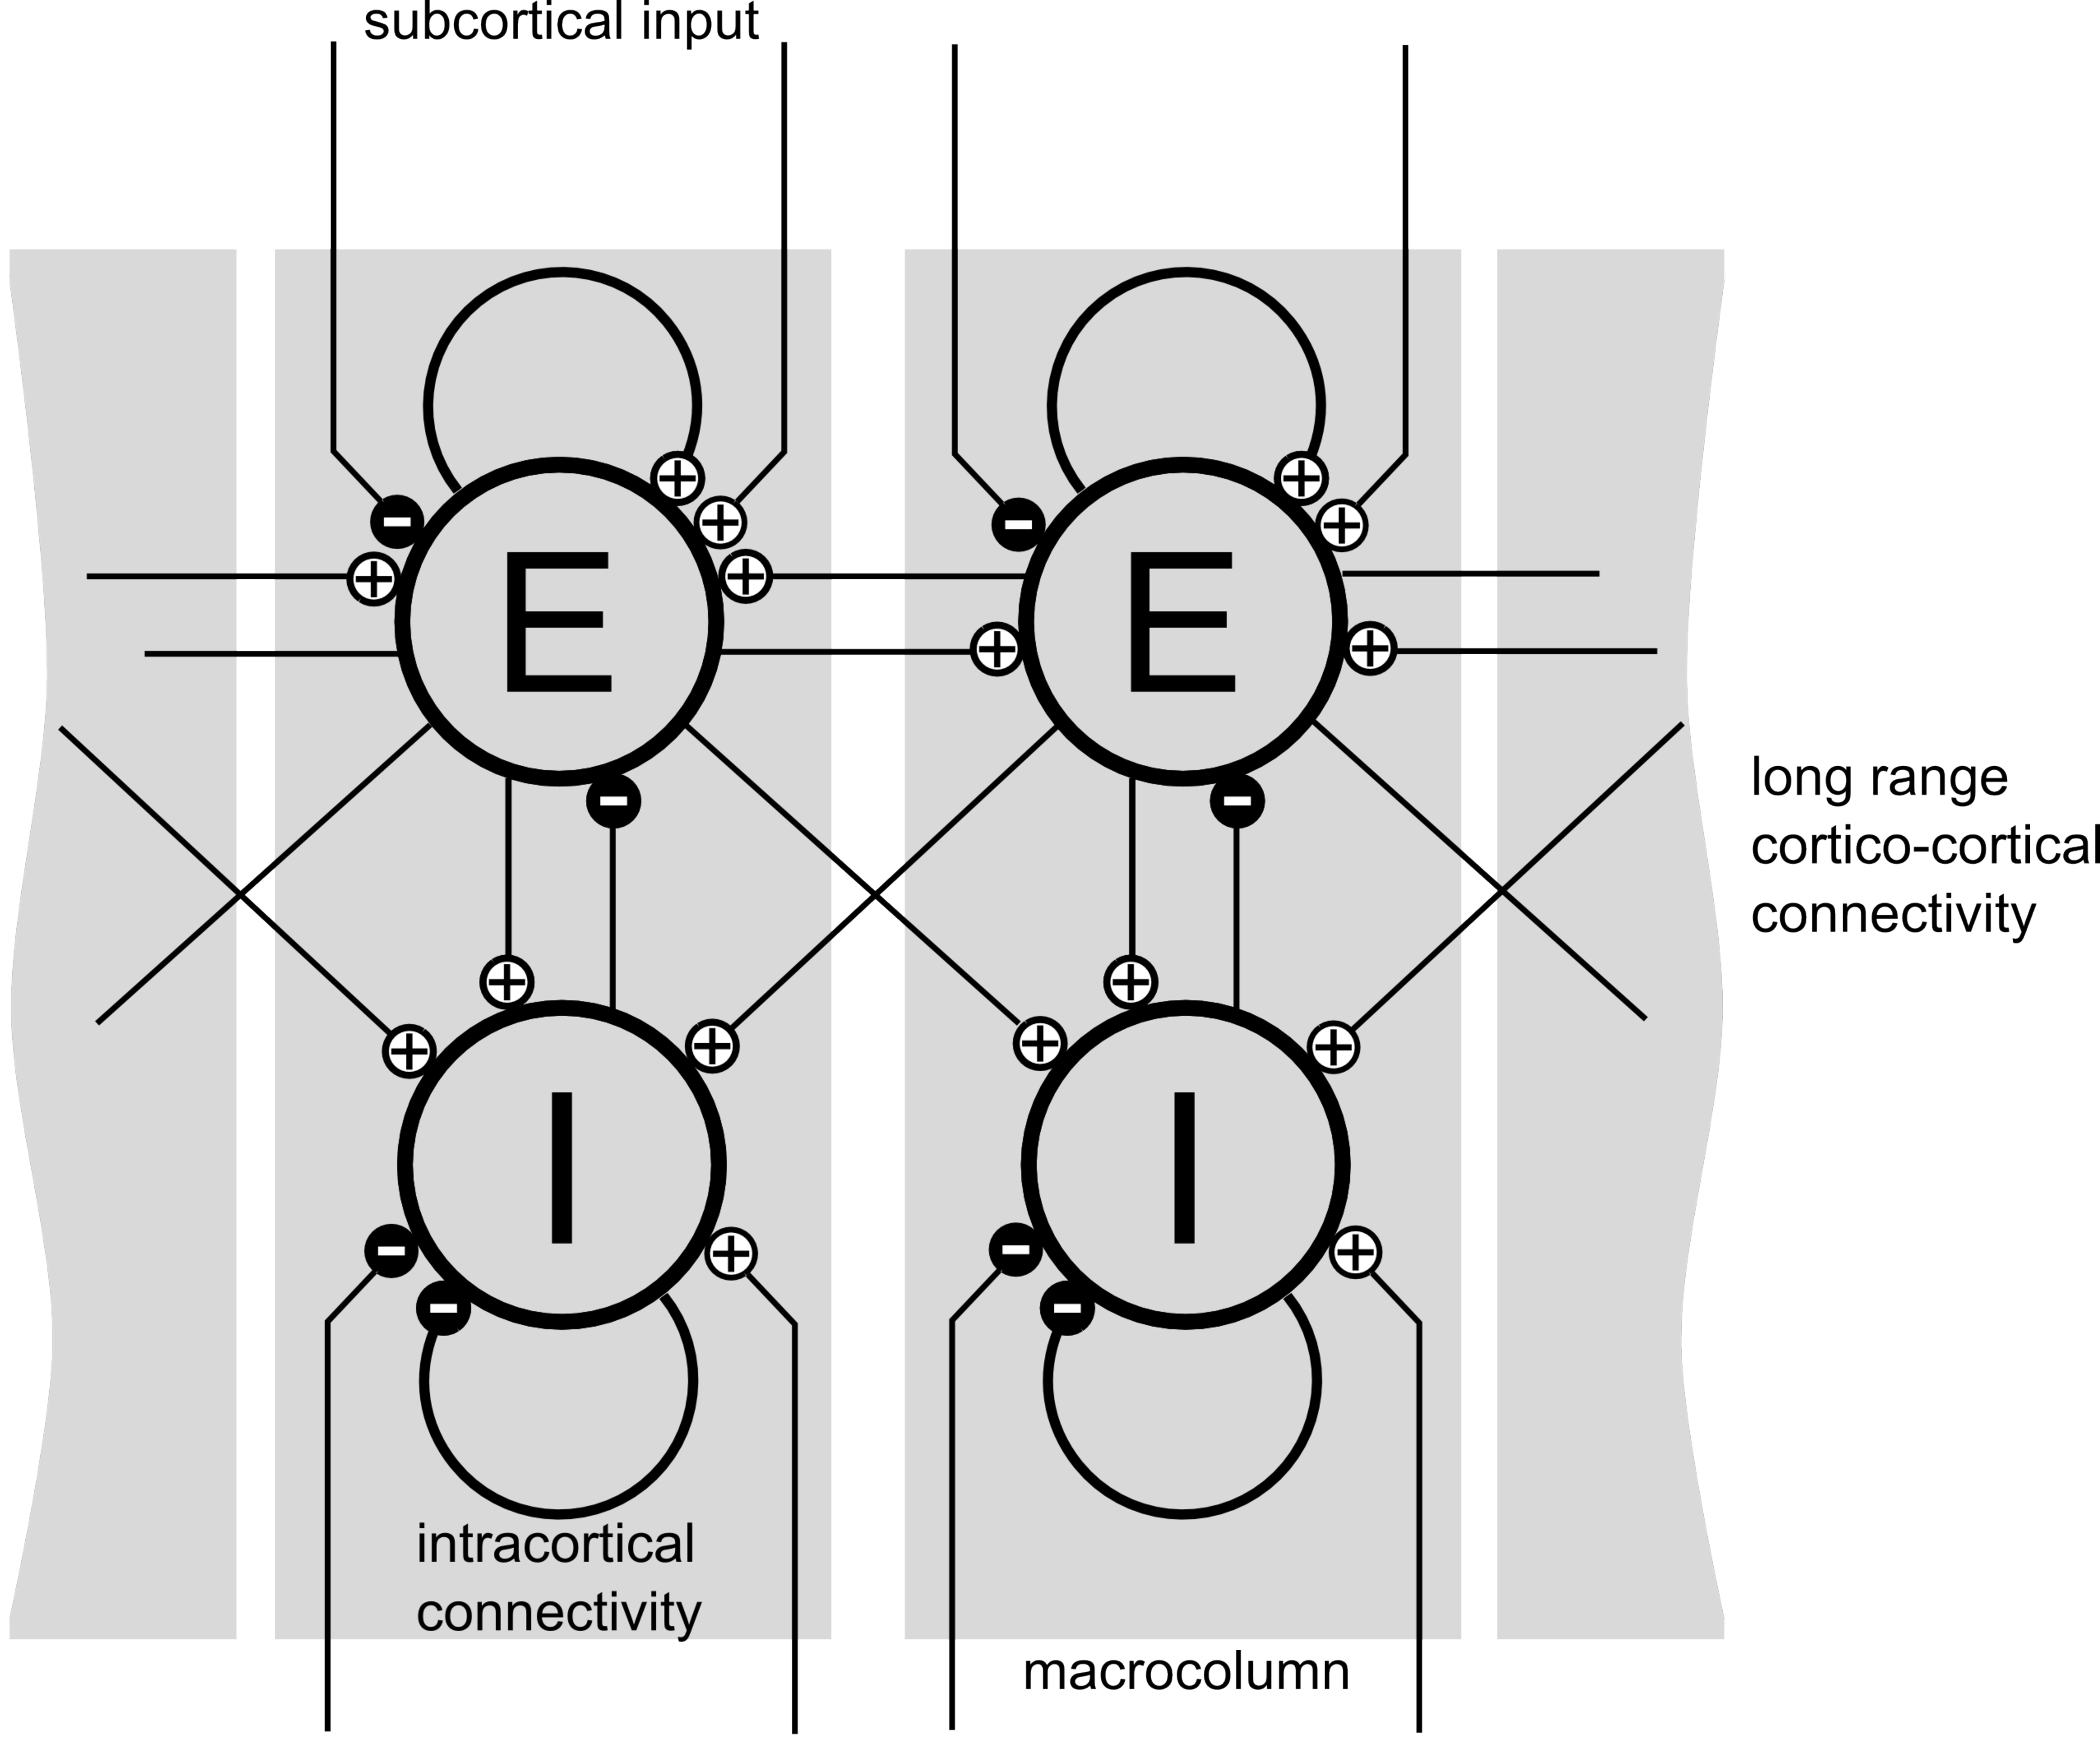
\includegraphics[scale=0.15]{chosen-frontiers-2012/liley_topology.pdf}
		\caption{Schematic overview of the essential intracortical and corticocortical
interactions between excitatory and inhibitory neuronal
populations in the model of Liley et al (2011; 2005; 2003; 2002;
1999). Figure reproduced with permission from Liley et al (2011).
Following conductance based approaches typically used to model
networks of synaptically interacting networks of individual model
neurons, excitatory and inhibitory neuronal populations are modeled as
single passive resistive-capacitive compartments into which all
synaptically induced postsynaptic currents flow. Functionally these
populations are equivalent to the excitatory and inhibitory KO sets of
Freeman’s (1975) K-set hierarchy. Cortical activity is then described
by the mean soma membrane potentials of the spatially distributed excitatory ($h_e$)
and inhibitory ($h_i$) neuronal populations. The connection with pysiological measurement is obtained through $h_e$,
which is
assumed to be linearly related to the surface recorded
electroencephalogram (Nunez \& Srinivasan, 2006; Freeman, 1975).}
\end{figure}

Thus the response of the mean soma membrane potential $h_k$ ($k=e,i$) at position $r$ on a two dimensional cortical
sheet, to induce post synaptic activity $I_{lk}$ ($l$=source, $k$=target population) is given by

\begin{equation} \label{eq:h_k} 
\tau_k\frac{\partial h_k(r,t)}{\partial t} = h^r_k - h_k(r,t) + \sum_{l=e,i} \frac{h_{lk}^{eq} - h_k(r, t)}{\left|
h_{lk}^{eq}-h_k^r\right|}I_{lk}(r,t)
\end{equation}

The postsynaptic response to a single pre-synaptic action potential (at
t = 0) is modeled by the well-known synaptic alpha function of cable
theory as $\Gamma_{lk} \gamma_{lk}texp(1-\gamma_{lk}t), t \geq 0$ and is excitatory or inhibitory depending
on the sign of $\Gamma_{lk}$ (peak amplitude), and thus we assume that the time
course of the synaptically induced excitatory and inhibitory currents is
described by a critically damped oscillator driven respectively by the
mean rate of incoming excitatory and inhibitory axonal pulses:

\begin{equation} \label{eq:i_lk}
\left( \frac{\partial}{\partial t} + \gamma_{lk} \right)^2 I_{lk}(r,t) = exp(1)\Gamma_{lk}\gamma_{lk}.A_{lk}(r,t)
\end{equation}

With
\begin{equation} \label{eq:a_ek}
A_{ek}(r,t) = N_{ek}^{\beta} S_e[ h_e(r,t)] + \phi_{ek} + p_{ek}(r,t)
\end{equation}

And
\begin{equation} \label{eq:a_ik}
A_{ik}(r,t) = N_{ik}^{\beta} S_i[h_i(r,t)] + p_{ik}(r,t)
\end{equation}

where $A_{lk}$ comprises the different sources of presynaptic spikes: $N_{lk}^\beta S_i$ (input from local cortical
neuronal populations), $\phi_{ek}$ (input from long range excitatory cortico-cortical fibres) and $p_{lk}$
(extracortical sources).
While the present consensus is that extracortical sources
(thalamocortical afferents) are purely excitatory in nature and thus $p_{ik} \cong 0$0, we choose to keep these terms as
they enable the effects of
tonic inhibition to be included without the need to define additional
parameters. The time courses of the synaptically induced currents, $1 / \gamma_{lk}$ are taken to describe the time
course of ‘fast’ excitatory ($l = e$: $\alpha$-amino-3-hydroxl-5-methyl-4-isoxazole-propionate (AMPA) \& kainate) and
inhibitory ($l=i$: $\gamma$-amino-butyric-acid type A (GABA\textsubscript{A}) neurotransmitter kinetics. Mean neuronal
population firing rates, $S_l$, are assumed to to instantanious sigmoid functions of the mean soma membrane potential
i.e

\begin{equation} \label{eq:s_l}
S_l[h_l(r,t)]=S_l^{max}/\{1 + exp[\sqrt{2}(h_l(r,t)-\mu_l)/\sigma_l]\}
\end{equation}

The axonal pulses $\phi_{ek}$ propagated by the exclusively excitatory long
range cortico-cortical fibre system is in the simplest case described by
the following two-dimensional telegraph equation,

\begin{equation} \label{eq:phi}
\left(\frac{\partial}{\partial t} + v_{ek} \Lambda_{ek} \right)^2 \phi(r,t) - \frac{3}{2} v_{ek}^2
\nabla^2\phi(r,t)=v_{ek}^2 \Lambda_{ek}^2 N_{ek}^\alpha S_e[h_e(r,t)]
\end{equation}

where $N_{ek}^\alpha$ is the total number of excitatory connections formed by
long range cortico-cortical axons on long on local population $k$, and
assumes a single axonal conduction velocity $v_{ek}$ and and an exponential fall
off with distance (characteristic scale = $1/\Lambda_{ek}$) of the strength of
cortico-cortical connectivity. For simplicity, and given the fact that in
anaesthesia burst suppression involves the whole brain, we chose to
only study the spatially homogeneous case i.e. $\nabla^2 = 0$

Equations (\ref{eq:h_k}, \ref{eq:i_lk}, \ref{eq:a_ek}, \ref{eq:a_ik} \& \ref{eq:phi}) represent a system of 8 coupled
non-linear partial
differential equations that typically defines the Liley model of
electrocortical rhythmogenesis, which is capable of reproducing the
main features of spontaneous human electroencephalogram (alpha
resonance, '$1/f$' activity). Table \ref{table:model_params} summarises all model parameters,
their definitions and approximate ranges. 

\begin{table}[h]
\label{table:model_params} 
\begin{tabular}{r l r r l}
\hline 
 & Definition & Min & Max & Units \\
\hline
$h_k^r$ & resting membrane potential & −80 & −60 & $mV$ \\
$\tau_k$ & passive membrane decay time & 5 & 150 & $ms$ \\
$h_{ek}^{eq}$ & excitatory reversal potential & −20 & 10 & $mV$ \\
$h_{ik}^{eq}$ & inhibitory reversal potential & −90 & $h_k^r - 5$ & $mV$ \\
$\Gamma_{ek}$ & EPSP peak amplitude & 0.1 & 2.0 & $mV$ \\
$\Gamma_{ik}$ & IPSP peak amplitude & 0.1 & 2.0 & $mV$ \\
$1/\gamma_{ek}$ & EPSP rise time to peak & 1 & 10 & $ms$ \\
$1/\gamma_{ik}$ & IPSP rise time to peak & 2 & 100 & $ms$ \\
$N_{ek}^\alpha$ & number of excitatory cortico-cortical synapses & 1000 & 5000 & − \\
$N_{ek}^\beta$ & number of excitatory intracortical synapses & 2000 & 5000 & − \\
$N_{ik}^\beta$ & number of inhibitory intracortical synapses & 100 & 1000 & − \\
$v_{ek}$ & axonal conduction velocity & 0.1 & 1 & $mm/ms$ \\
$1 / \Lambda_{ek}$ & decay scale cortico-cortical connectivity & 10 & 100 & $mm$ \\
$S_k^{max}$ & maximum firing rate & 0.05 & 0.5 & $ms^{-1}$ \\
$\mu_k$ & mean firing threshold & −55 & −40 & $mV$ \\ 
$\sigma_k^2$ & variance in firing threshold & 4 & 49 & $mV^2$ \\
$p_{lk}$ & extracortical synaptic input rate & 0 & 10 & $ms^{-1}$ \\
\hline
\end{tabular}
\caption{List of spatially averaged parameters for different types $k = e,
i$ of neuronal target populations in the electrocortical model of Liley et
al. (2011; 2005; 2003; 2002; 1999), with typical ranges that are
assumed to be physiologically admissible. Table adapted from Liley et
al (2011).}
\end{table}

\subsection{Model parameterisation: generation of normative parameter sets}
Because burst suppression activity (at least that caused by
anaesthetic and sedative action) is assumed to ultimately arise out of
a background of normal electroencephalographic activity it is
important to define parametrically normative states in order to study
how they may be perturbed during health and disease. We therefore
chose to utilize previously defined parameter sets (Bojak \& Liley,
2005) that have the following properties: i) are confined to the
physiologically admissible parameter space (see Table 1), ii) give rise
to electroencephalographically and physiologically plausible activity
('1/f' decay at low frequencies plus a relatively sharp peak at alpha
frequencies, 8 – 13 Hz; mean excitatory/inhibitory neuronal firing rates
< 20 $s^{-1}$) and iii) that exhibit transient increases in total power and
monotonic reductions in mean frequency with respect to modeled
anaesthetic action (see below). In general such sets are found by
randomly searching the high dimensional physiologically admissible
(and plausible) parameter space. For further details see Bojak \& Liley
(2005).

\begin{table}[h]
\label{table:site_of_action} 
\begin{tabular}{p{5cm} p{5cm} l}
\hline 
 Site of action & Main anaesthetic effect & Parameters \\
\hline
2PK channels \& extrasynaptic GABA$_A$ receptors & increase in tonic inhibition & $p_{ik}, h_k^r$ \\
\\
HCN1 pacemaker channels & membrane hyperpolarisation, increase in EPSP amplitude$^a$ & $\Gamma_{ee}, h_e^r$\\
\\
nACh receptors & reduction in tonic excitation & $p_{ek}, h_k^r$ \\
\\
synaptic GABA$_A$ & increase in IPSP charge transfer & $\Gamma_{ik}, \gamma_{ik}, \epsilon_{ik}$\\
\\
AMPA/kainate \& NMDA$_b$ receptors & decrease in EPSP charge transfer & $\Gamma_{ek}, \gamma_{ek}, \epsilon_{ek}$\\
\\
myelinated axons$^c$ & decreased conduction velocity & $v_{ek}$\\
\\
Na channels & alterations of neuronal firing & $S_k^{max}, \mu_k, \phi_k$\\
\hline
\end{tabular}
\caption{Relationship between major experimentally identified sites of
cortical anaesthetic action and parameters of the electrocortical model
of Liley et al. (2005; 2003; 2002; 1999). EPSP = excitatory
postsynaptic potential; IPSP = inhibitory postsynaptic potential; 2PK =
two-pore potassium; nACh = nicotinic acetylcholinergic; NMDA = Nmethyl-
d-aspartate; $^a$ only demonstrated in excitatory neurons (Chen
et al, 2009). $^b$ hypothesized to depend on $h_k$ ; $^c$ Effect demonstrated
in periphery, speculative in cortex (Swindale, 2003). Table adapted
from Liley et al (2011).}
\end{table}



\subsection{Investigating and incorporating speculative physiological
mechanisms of burst suppression}
While it is often assumed that burst-suppression pattern arises from
slow thalamic oscillations driving cortex (Fisch, 1999), the fact that
this pattern persists subsequent to cortical deafferentation instead
suggests that it is an intrinsic dynamical feature of cortical tissue
(Luktach et al, 1995).
While many anaesthetic agents, at sufficiently high doses, are capable
of producing burst suppression pattern electroencephalogram, not all
do. Pharmacologically, anaesthetics that induce burst suppression all
seem to have a GABAergic profile, even if weak. One that has not
been reported to induce burst suppression, xenon, is widely believed to
act principally via the antagonism of glutamatergic neurotransmission.
Indeed it is reported in laboratory slice preparations that burst
suppression induced by thiopental, propofol and isoflurane requires the
maintenance of glutamate-mediated excitatory neurotransmission
(Luktach et al, 2005). While NMDA antagonists have been shown to
reduce burst duration and amplitude in slice preparations (Kroeger \&
Amzica, 2007), in clinical practise antiepileptic drugs generally show
poor response.
Lukatch \& MacIver (1996) report that burst suppression appears to
result from the direct activation of GABA-gated Cl– channels as
muscimol, a potent selective GABAA agonist, reliably induces this
phenomenon. Therefore perturbation of GABAergic neurotransmission
may be key to understanding the pathophysiology of burst
suppression. Such a view is also supported by work involving
hippocampal slices subject to simulated ischemia in which it is found
that ischemia releases GABA initially by exocytosis and then by
reversal of a high affinity GABA plasma membrane transporter (GAT-1;
Allen et al, 2004).
The implied importance of GABAergic inhibitory processes is also
supported by the work of Steriade et al (1994) in which they found
that hyperpolarisation of the resting cell membrane potential of
cortical neurons reliably preceded conspicuous electroencephalographic
aspects of burst suppression. However in addition to inhibitory
GABAergic contributions they also ascribed the hyperpolarisation to i)
thalamic disfacilitation ii) inactivation of a variety of inward ionic
currents and iii) increases in membrane K+ conductances.
While maintenance of a sufficient level of glutamate-mediated
excitatory neurotransmission is required for the genesis of the bursting
in burst suppression, there is nevertheless evidence that
neurotransmission in general is attenuated. For example Kroeger \&
Amzica (2007) showed that bursting depleted interstitial Ca2+ to a
level incompatible with synaptic transmission, and speculate that this
accounts for the isoelectric suppression period. That attenuated
neurotransmission may also be involved in the genesis of hypoxia
induced burst suppression is supported by the works of Endemli and
Crunelli (1998), in which they found that brief periods of anoxia can
cause a total, but reversible loss of synaptic transmission, and
Fleidervish et al (2001), in which it was found that hypoxia depleted
readily releasable pools of vesicles for transmitter release.

\subsection{Theoretical basis of busrting}
Bursting is generally characterised by oscillations occurring on two different time scales \cite{izikevich2007_1}. Fast
oscillations underlie the active phase of bursting and slow oscillations underlie the quiescent periods of suppression. These systems are generally coupled with the fast system feeding in to the slow subsystem and the slow subsystem feeding back in to the fast.

The difference of timescales between the fast subsystem and slow subsystem must be significant. If $\tau^{fast}$ is the characteristic timescale for the fast subsystem and $\tau^{slow}$ is the characteristic timescale for the slow subsystem then $\tau^{fast}/\tau^{slow} \ll 1$ for it to be considered a fast/slow system.

\subsection{Fast dynamics within the model of Liley et Al}
Liley et al (Liley et al, 2003 - Drug-induced modification of the system properties associated
with spontaneous human electroencephalographic activity) propose that oscillatory activity within cortical interneuron
(inhibitory) circuits is generated by a feedback mechanism between the excitatory and inhibitory population.
The inhibitory population activity phase leads excitatory population activity, generating a phase locked system of
inhibitory and excitatory neurons generating the observed oscillatory behaviour.

The phase locking of these systems leads us to assume that equations \ref{eq:h_k} and \ref{eq:i_lk} represent a single
timescale within the model of Liley et al and as therefore were considered as together to be a 'fast' system for this
exploration.

\subsection{Introduction of a mean field averaging system}

We began by introducing a generalised mean field averaging system $\zeta_{k}, k \in \{e, i\}$.  $\zeta_{k}$ represents a low pass filtering of the mean field $h_k$ and is driven by the mean field proportionally to its firing rate $s_{k}(h_{k})$.

A simple first order low pass filter was used for $\zeta_k$, represented by the following coupled ordinary differential equation

\begin{equation} \label{eq:zeta_slow} 
\tau_k^{slow} \frac{\partial \zeta_k}{\partial t} = g_k s_k(h_k) - \zeta_k
\end{equation}
where $\tau_j^{slow}$ is the time constant for the slow system and $g_k$ the mean field connectivity
constant (UNITS).

$\zeta_{k}$ was used to augment the cannonical equations of the Liley et al model. These augmentations were used to investigate several physiologically plausible fast/slow topologies for burst suppression.

\subsection{Modelling thalamic averaging of the mean field}
Cortico-Thalamic feedback has been proposed as a mechanism for the generation of slow sleep waves (ref steriade etc). 
We investigated the plausibility of such a system driving BS. 

We augmented the cannonical model of Liley et al. to introduce a a cortico-thalamic feedback component. 
In (\ref{eq:a_ek}) $p_{ek}$ is a constant representing the rate of extra cortical input. Modelling cortico-thalamic feedback, $p_{ek}$ was reformulated to include a slow deviation from its resting value that was proportial to $\zeta_e$. The constants for $p_{ek}$ in (\ref{eq:a_ek}) were replaced with the expression

\begin{equation} \label{eq:p_ek}
p_{ek} = \hat{p_{ek}} - \rho_{ek} \zeta_e
\end{equation}

$\rho_{ek}$(UNITS!!) is a constant of proportionality to $\zeta_e$, representing the amount of thalamic feedback connectivity. $\hat{p_{ek}}$ is a constant, representing
the resting value for the rate of extra cortical input, corresponding to the original constant expression for $p_{ek}$ in the cannonical model. 

It should be noted in this case that when $\rho\zeta_e=0; \forall t \geq 0$ this augmented model collapses to the cannonical model of Liley et al.

\subsection{Modelling intracellular and/or synaptic resource utilisation}
(Tsodyks and Markram 1997, Bazhenov et Al 2002) introduced generic models of synaptic resource utilisation and recovery that depend
on neuronal activity. We introduced a model of intracellular and synaptic resource depletion to account for the expenditure of the resources utilised by neuronal and synaptic activity. 

It was assumed that a depletion in intracellular or synaptic resources would present itself as a decrease in the peak PSP. Therefore we reformulated the excitatory PSPs ($\Gamma_{ee}, \Gamma_{ei}$) to
account for intracellular/synaptic resource depletion and recovery.

The effect that intracellular/synaptic resource utilisation and recovery has on the peak PSP was assumed to be proportial to the generic averaging system $\zeta_{e}$, giving an expression for
the excitatory PSPs:

\begin{equation} \label{eq:Gamma_ek}
\Gamma_{ek} = \hat{\Gamma_{ek}} - \chi_{ek} \zeta_e
\end{equation}

Where $\hat{\Gamma_{ek}}$ is the original constant expression for $\Gamma_{ek}$, representing the resting post synaptic potential. $\chi$ is a constant of proportionality between $\zeta_e$ and the utilisation of intracellular resources (UNITS!!).

Again, it should be noted that when $\chi_{ek} \zeta_e=0; \forall t \geq 0$ this augmented model collapses to the cannonical model of Liley et al.

\subsection{Emergence of a slow system from a parametric variation of long range coupling constants}
The possibility of the long range coupling $\phi_{ek}$ operating on a timescale slower than that of the coupled excitatory/inhibitory system was investigated. If a slow system is able to emerge from the long range coupling, then it could be a possible contributor to BS. 

Swindale 2003 proposes that anaesthesia may bring about changes to axonal conduction velocities and capacitances. We investigated the
effects of modifying the conduction velocity and the characteristic decay scale ($v$ and $1 / \Lambda_{ek}$) had on the
long range coupling $\phi_{ek}$ system. The investigation looked at the ability of the long range coupling the to operate on a timescale slower than the coupled excitatory/inhibitory system and thus bringing about about BS.

\subsection{Parametric variation of fast system parameters}
GABAergic anaesthetics are known to predominantly affect the inhibitory system. We studied the dynamical effect of varying model parameters that are known to vary under the effect of GABAergic anaesthetics, namely $\Gamma_{ik}$, $\tau_i$ and $\gamma_{ik}$. We studied the effects of varying these parameters within any parameter sets that were found to exhibit BS.

\subsection{Identification of BS candidate parameter sets}
Riznel (1995) introduces a method of dissection to analyse bursting. The fast and slow systems are considered separately and the slow system can be frozen, replacing it with a parameter in the fast system. The frozen system can be used to analyse the dynamics of the fast system with respect to the slow system's value. Izhikevich (ref) introduces common bursting topologies, where the transitions between quiescence and spiking can be viewed as bifurcations with respect to the slow parameter(s).

A large scale numerical bifurcation analysis was performed on previously generated parameter sets(ref to sets). The slow system for each investigation was frozen with the frozen parameter being used as the free parameter within the bifurcation analysis. Parameter sets that displayed a topological liklihood of supporting BS were investigated individually. With the parameter sets that displayed a liklihood of bursting various slow system time constants and coupling terms $\tau_k^{slow}, g_k, \chi_{ek}, \rho_{ek}, v$ and $1 / \Lambda_{ek}$ were trialled in an attempt to produce BS.

\subsection{Computational methods}
All numerical integrations and bifurcation analysis of the aforementioned models were performed using the Python programming language, utilising
the PyDSTool library (available from \url{http://sourceforge.net/projects/pydstool/}) running under 64 bit
Linux. The Radau integrator that comes standard with PyDSTool was used for all integrations.
Typical numerical settings used for the radau integrator were $init\_step = 1e-6$, $atol = 1e-15$, $rtol = 1e-16$ and
$max\_pts = 40000000$.

\section{Results}

\subsection{Burst suppression arises in all investigated models}
A large scale numerical bifurcation analysis of existing parameter sets was performed for each of the models under investigation. For the model of thalamic averaging and the model of synaptic and intracellular resource utilisation $\zeta_e$ was frozen and used as a bifurcation parameter. For the cannonical model of Liley et al., $\phi_{ei}$ and $\phi_{ee}$ were frozen and were replaced with a single bifurcation parameter $\phi$. These analyses identified candidate parameter sets that displayed topologies that could support bursting.

We individually examined candidate parameter sets by varying appropriate slow system parameters. For the models of synaptic/intracellular resource utilisation and the model of thalamic averaging we trialled values for $\tau^{slow}_e$, their respective coupling factors ($\chi_{e}$, $\rho_{e}$) and by setting $g_e=0.7$. Within the cannonical model we trialed values for $v_{ei}$ and $\Lambda_{ei}$.

All three models displayed BS under appropriate parametric conditions. Slow oscillations in $\zeta_e$ were seen to emerge along with BS, in both the model of thalamic averaging and the model of synaptic/intracellular resource utilisation (see figure \ref{fig:emerging_slow_zeta}). Slow oscillations in $\phi_{ei}$ also emerged with BS (see figure \ref{fig:phi_dyn}). We found that the dynamics of ($\phi_{ei}$) were able to operate on a timescale slower and independent to that of the coupled (fast)
excitatory/inhibitory system (see figure \ref{fig:phi_dyn}), making it the slow system underlying the observed BS.

In all three models we altered fast system parameters $\gamma_{ik}, \tau_i$ and $\Gamma_{ik}$ on the parameter sets that were discovered to display BS.  The parametric alterations showed that bursting dynamics were highly variable with respect to the fast system parameters, with transitions between tonic spiking and BS being triggered by alterations in fast system parameters alone(see figure \ref{fig:00143}, \ref{fig:intra_gamma}, \ref{fig:phi_fast_var}).

\begin{figure}
	\begin{subfigure}[b]{0.5\textwidth}
		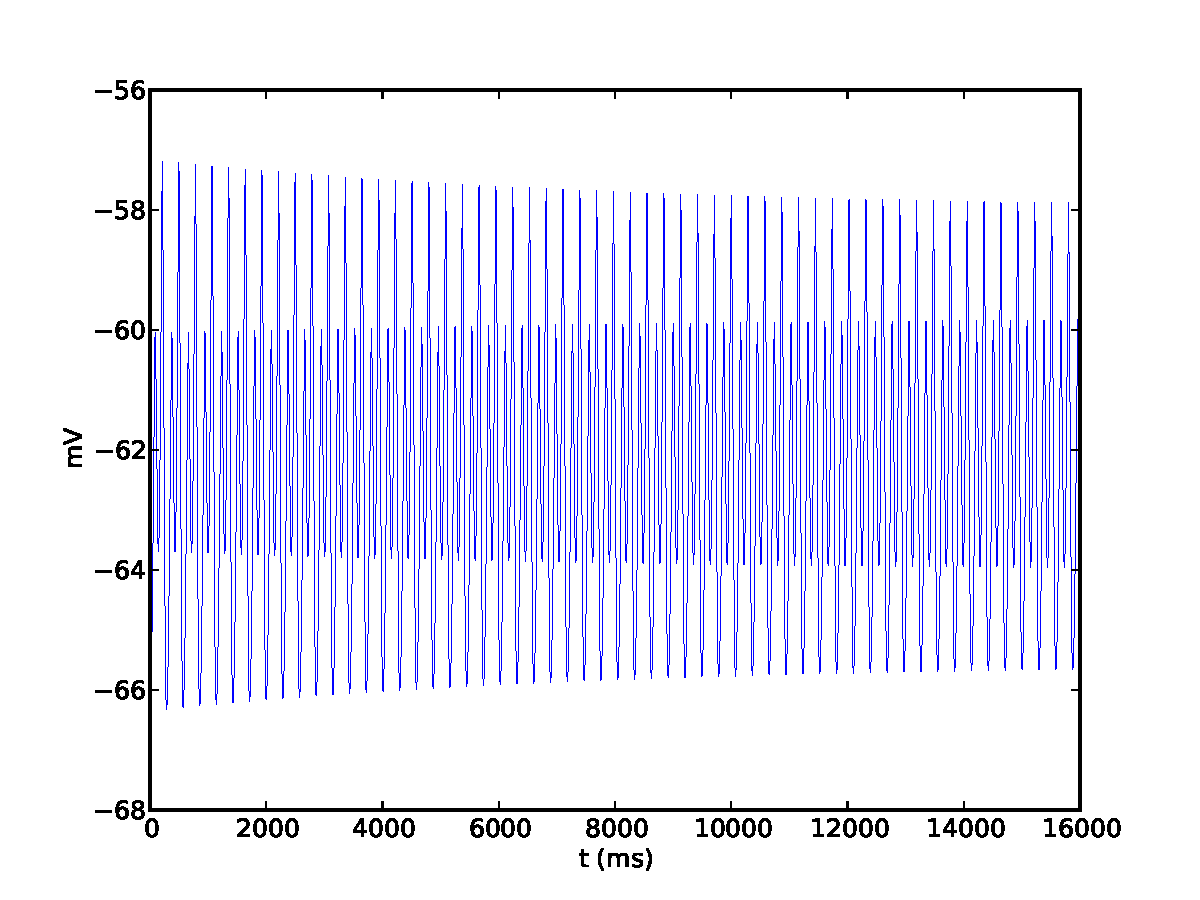
\includegraphics[scale=0.35]{chosen-frontiers-2012/00143-1-1-6-he-thal.pdf}
		\label{fig:00143_a}
		\caption{$h_e (mV)$}
	\end{subfigure}
	\begin{subfigure}[b]{0.5\textwidth}
		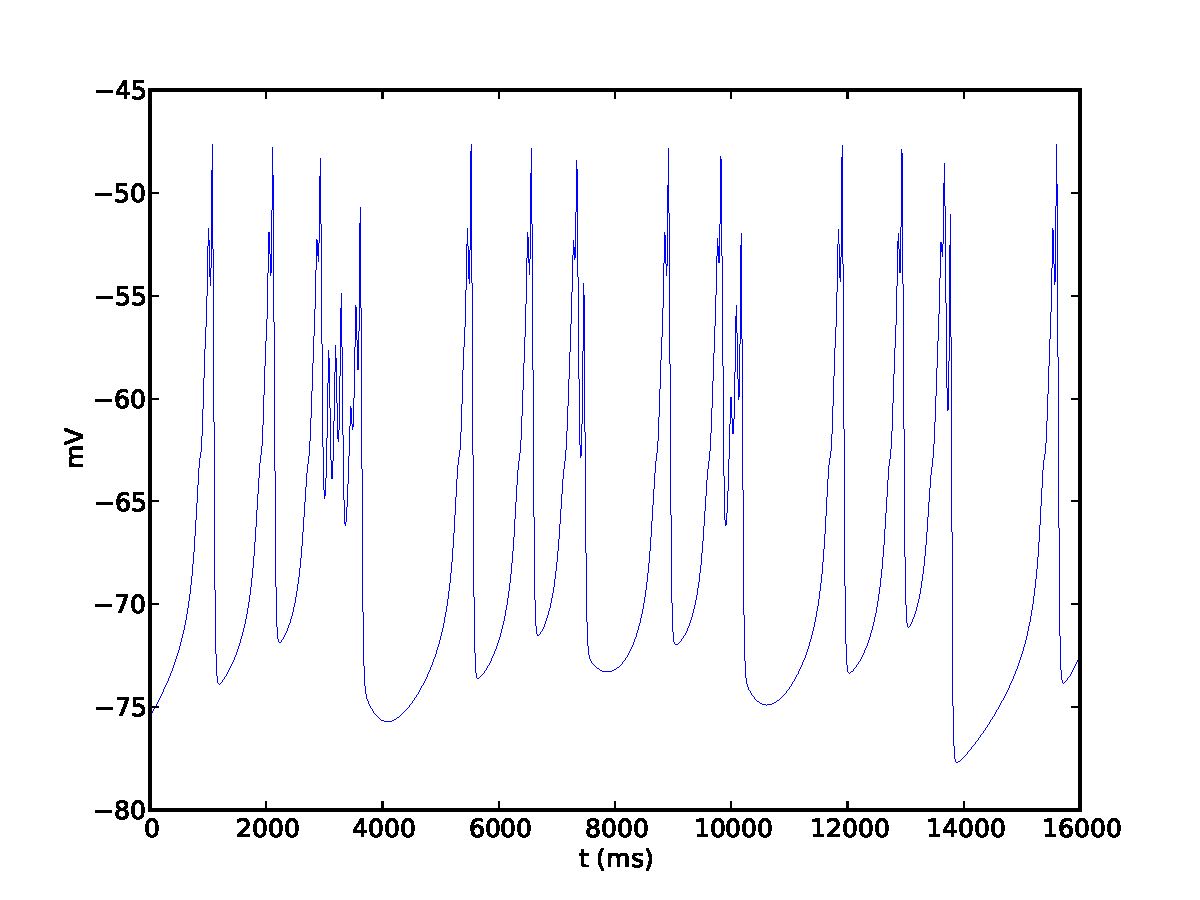
\includegraphics[scale=0.35]{chosen-frontiers-2012/00143-1_2-1-6-he-thal.pdf}
		\label{fig:00143_b}
		\caption{$h_e (mV)$}
	\end{subfigure}
	\begin{subfigure}[b]{0.5\textwidth}
		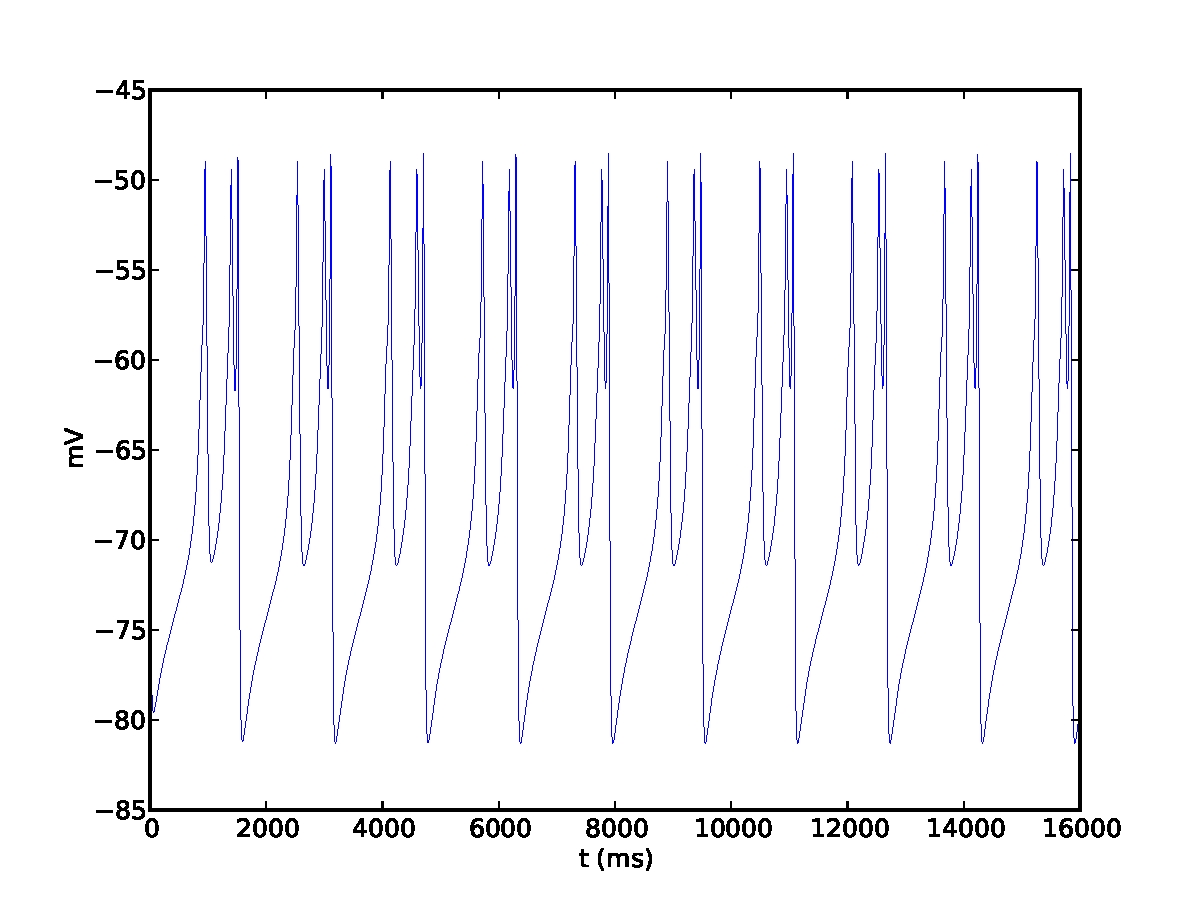
\includegraphics[scale=0.35]{chosen-frontiers-2012/00143-1-0_4-6-he-thal.pdf}
		\label{fig:00143_c}
		\caption{$h_e (mV)$}
	\end{subfigure}
	\begin{subfigure}[b]{0.5\textwidth}
		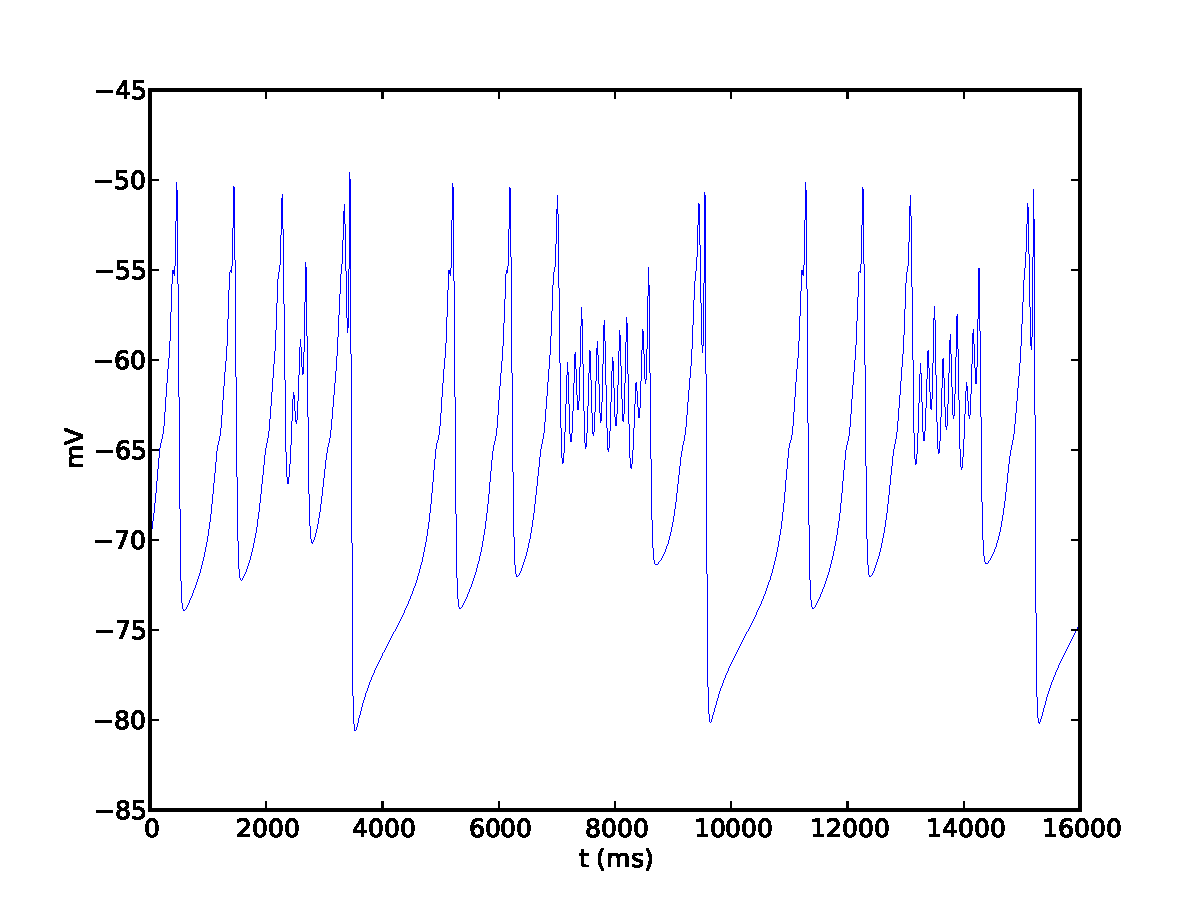
\includegraphics[scale=0.35]{chosen-frontiers-2012/00143-1-1-5-he-thal.pdf}
		\label{fig:00143_d}
		\caption{$h_e (mV)$}
	\end{subfigure}
	\label{fig:00143}
	\caption{Effect of varying fast system parameters $\gamma_{ie}$, $\gamma_{ii}$, $\Gamma_{ie}$, $\Gamma_{ii}$ and $\tau_i$ with the model of thalamic averaging\\
\\
a. $\gamma_{ie} = 0.06603578$, $\gamma_{ii} = 0.05208962$, $\Gamma_{ie} = 1.39744992$, $\Gamma_{ii} = 1.38041254$ and $\tau_i = 135.1578$ \\
b. $\gamma_{ie} = 0.079242936$, $\gamma_{ii} = 0.062507544$, $\Gamma_{ie} = 1.39744992$, $\Gamma_{ii} = 1.38041254$ and $\tau_i = 135.1578$ \\
c. $\gamma_{ie} = 0.06603578$, $\gamma_{ii} = 0.05208962$, $\Gamma_{ie} = 0.558979968$, $\Gamma_{ii} = 0.552165016$ and $\tau_i = 135.1578$ \\
d. $\gamma_{ie} = 0.06603578$, $\gamma_{ii} = 0.05208962$, $\Gamma_{ie} = 1.39744992$, $\Gamma_{ii} = 1.38041254$ and $\tau_i = 112.6315$ \\
\\
All other parameters are:\\
$\Lambda_{ee}: 0.97960647, \Lambda_{ei}: 0.97960647, N^{\alpha}_{ee}: 3218.25773139, N^{\alpha}_{ee}: 1725.76994483,
N^{\beta}_{ee}: 2555.55531967, N^{\beta}_{ei}: 3955.4019654, N^{\beta}_{ie}: 558.83565101, N^{\beta}_{ii}: 805.76418084,
\Gamma_{ee}: 0.15172837, \Gamma_{ei}: 0.27123796, 
g_e: 0.7, \gamma_{ee}: 0.31475255879, \gamma_{ei}: 0.24594817, h^{rest}_e: -66.96584987, h^{eq}_{ee}: 0.0353266, h^{eq}_{ei}: -6.84352222,
h^{rest}_i: -77.90610838, h^{eq}_{ie}: -85.52639408, h^{eq}_{ii}: -85.434985,
\mu_e: -50.73253197, \mu_i: -51.66219544, \hat{p_{ee}}: 2.1687293948, \hat{p_{ei}}: 2.4342247579, p_{ie}: 0.0, p_{ii}: 0.0, \phi_{ie}: 0,
\phi_{ii}: 0, S^{max}_e: 0.101903, S^{max}_i: 0.469, \sigma_e: 6.02438944, \sigma_i: 4.21865921,
\rho_e: 2000.0, \rho_i: 2000.0, \tau_e: 139.779, \tau_i: 135.1578, \tau^{slow}: 6988.95,
  v_{ee}: 0.681401, v_{ei}: 0.681401$
}
\end{figure}

\begin{figure}
	\begin{subfigure}[b]{0.5\textwidth}
		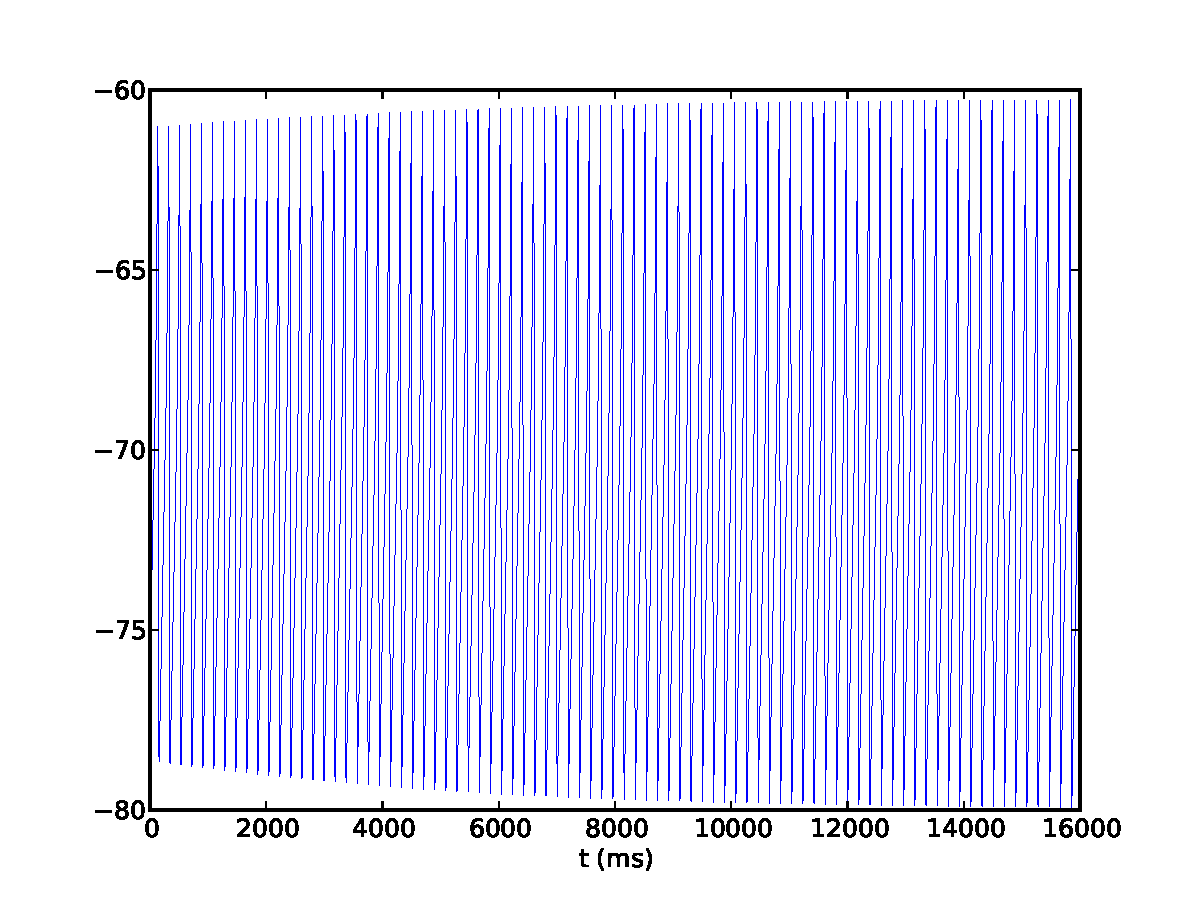
\includegraphics[scale=0.35]{chosen-frontiers-2012/00493-1-he-intra.pdf}
		\label{fig:493_a}
		\caption{$h_e (mV)$}
	\end{subfigure}
	\begin{subfigure}[b]{0.5\textwidth}
		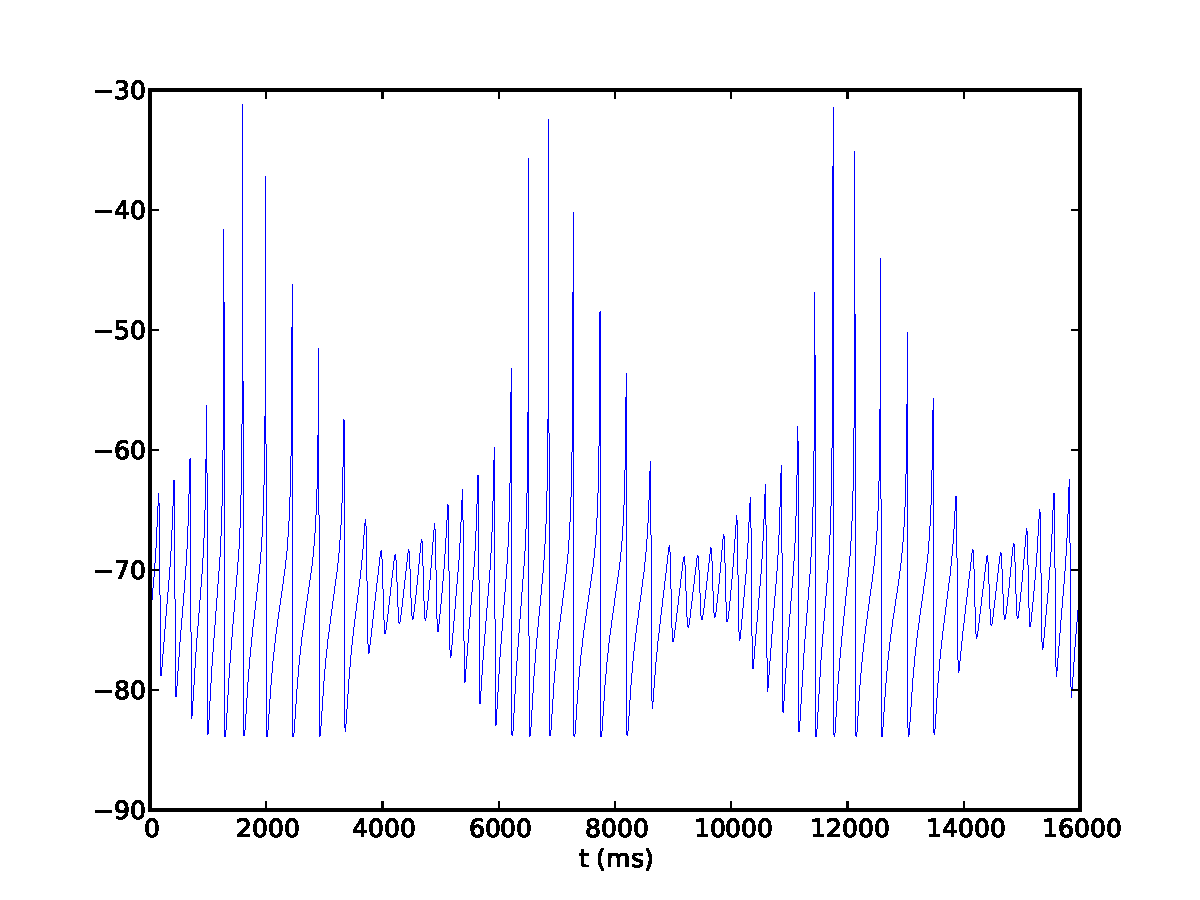
\includegraphics[scale=0.35]{chosen-frontiers-2012/00493-0_5-he-intra.pdf}
		\label{fig:493_b}
		\caption{$h_e (mV)$}
	\end{subfigure}
	\begin{subfigure}[b]{0.5\textwidth}
		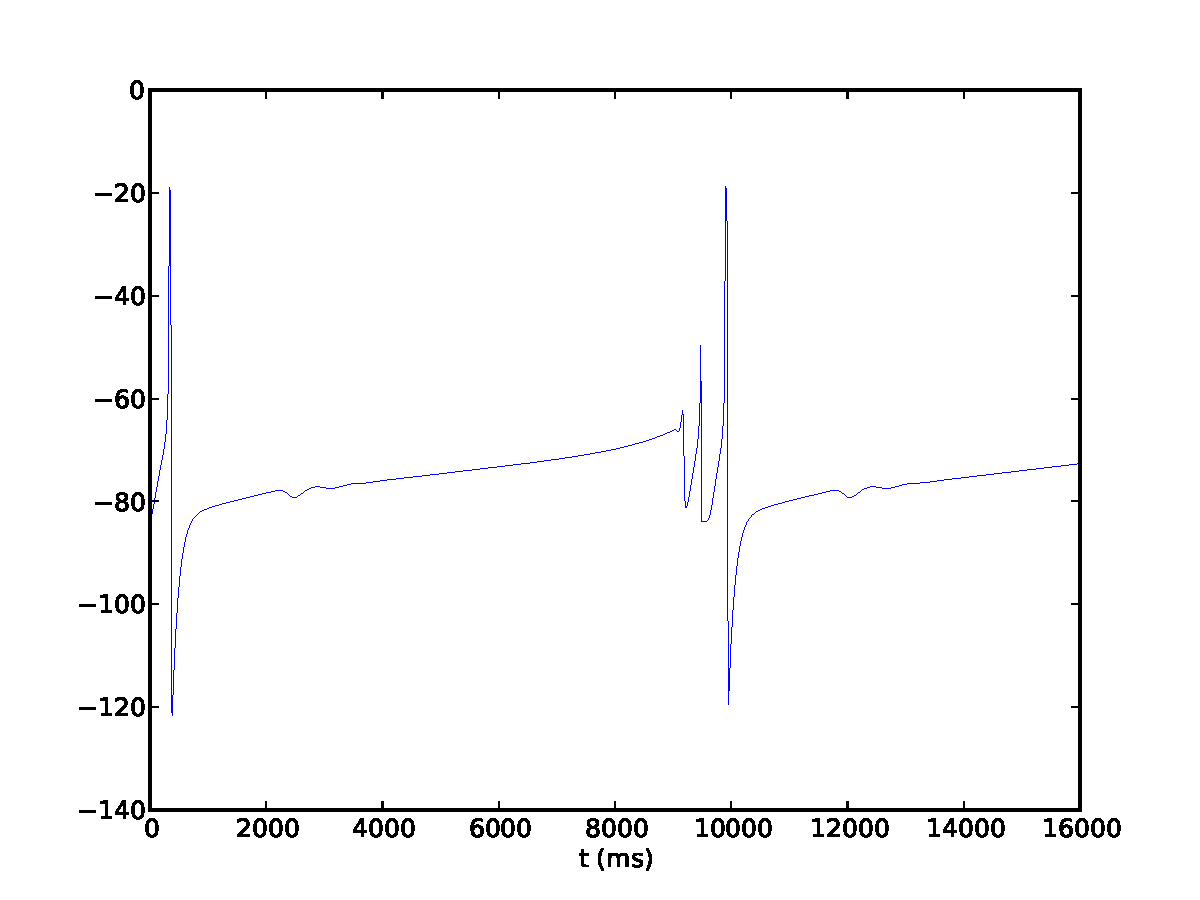
\includegraphics[scale=0.35]{chosen-frontiers-2012/00493-0_11-he-intra.pdf}
		\label{fig:493_c}
		\caption{$h_e (mV)$}
	\end{subfigure}
	\begin{subfigure}[b]{0.5\textwidth}
		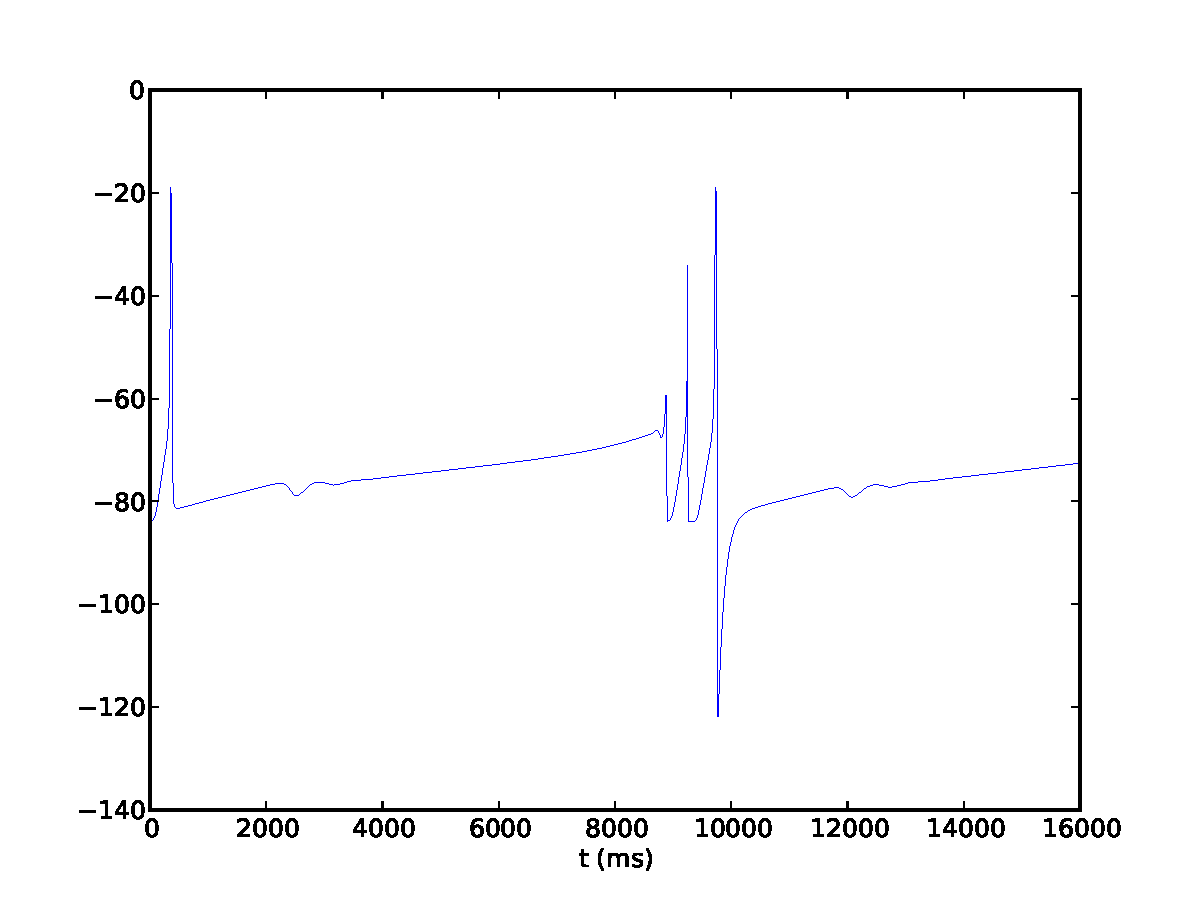
\includegraphics[scale=0.35]{chosen-frontiers-2012/00493-0_1-he-intra.pdf}
		\label{fig:493_d}
		\caption{$h_e (mV)$}
	\end{subfigure}

	\label{fig:intra_gamma}
	\caption{The effects of varying fast system parameters $\gamma_{ie}$ and $\gamma_{ii}$ with the model of synaptic/intracellular resource utilisation. \\
	Values for $\gamma_{ie}, \gamma_{ii}$ are as follows: \\
\ref{fig:493_a}: $\gamma_{ie}=0.51495496832$, $\gamma_{ii}=0.03891608$ \\
\ref{fig:493_b}: $\gamma_{ie}=0.25747748416$, $\gamma_{ii}=0.01945804$ \\
\ref{fig:493_c}: $\gamma_{ie}=0.0566450465152$, $\gamma_{ii}=0.0042807688$ \\
\ref{fig:493_d}: $\gamma_{ie}=0.051495496832$, $\gamma_{ii}=0.003891608$ \\
All other parameters:\\ \\
$\Lambda_{ee}: 0.861765043, \Lambda_{ei}: 0.861765043, N^{\alpha}_{ee}: 2564.793282, N^{\alpha}_{ei}: 1118.08004, N^{\beta}_{ee}: 3745.711734, N^{\beta}_{ei}: 3144.983978, N^{\beta}_{ie}: 446.4477283, N^{\beta}_{ii}: 345.8866865, \Gamma_{ee}: 1.6861042005, \Gamma_{ei}: 1.885871361, \hat{\Gamma_{ie}}: 5.855116285, \hat{\Gamma_{ii}}: 6.9331585350000005, g_e: 0.7, \gamma_{ee}: 0.95083473, \gamma_{ei}: 0.79156622, \chi_{ee}: 700.0, \chi_{ei}: 700.0, h^{rest}_e: -79.61058688, h^{eq}_{ee}: -17.9914286, h^{eq}_{ei}: -15.53827744, h^{rest}_i: -71.24328917, h^{eq}_{ie}: -84.00936425, h^{eq}_{ii}: -89.797995, \mu_e: -41.12042539, \mu_i: -54.45064422, p_{ee}: 2.6864898634, p_{ei}: 6.648040185, p_{ie}: 0.0, p_{ii}: 0.0, \phi_{ie}: 0, \phi_{ii}: 0, r^{abs}: 0.0, S^{max}_e: 0.400558, S^{max}_i: 0.404191, \sigma_e: 6.55747395, \sigma_i: 2.047597811, \tau_e: 108.758, \tau_i: 232.0, \tau^{slow}_e: 5437.9, v_{ee}: 0.419426, v_{ei}: 0.419426$
}
\end{figure}

\begin{figure}
	\begin{subfigure}[b]{0.5\textwidth}
		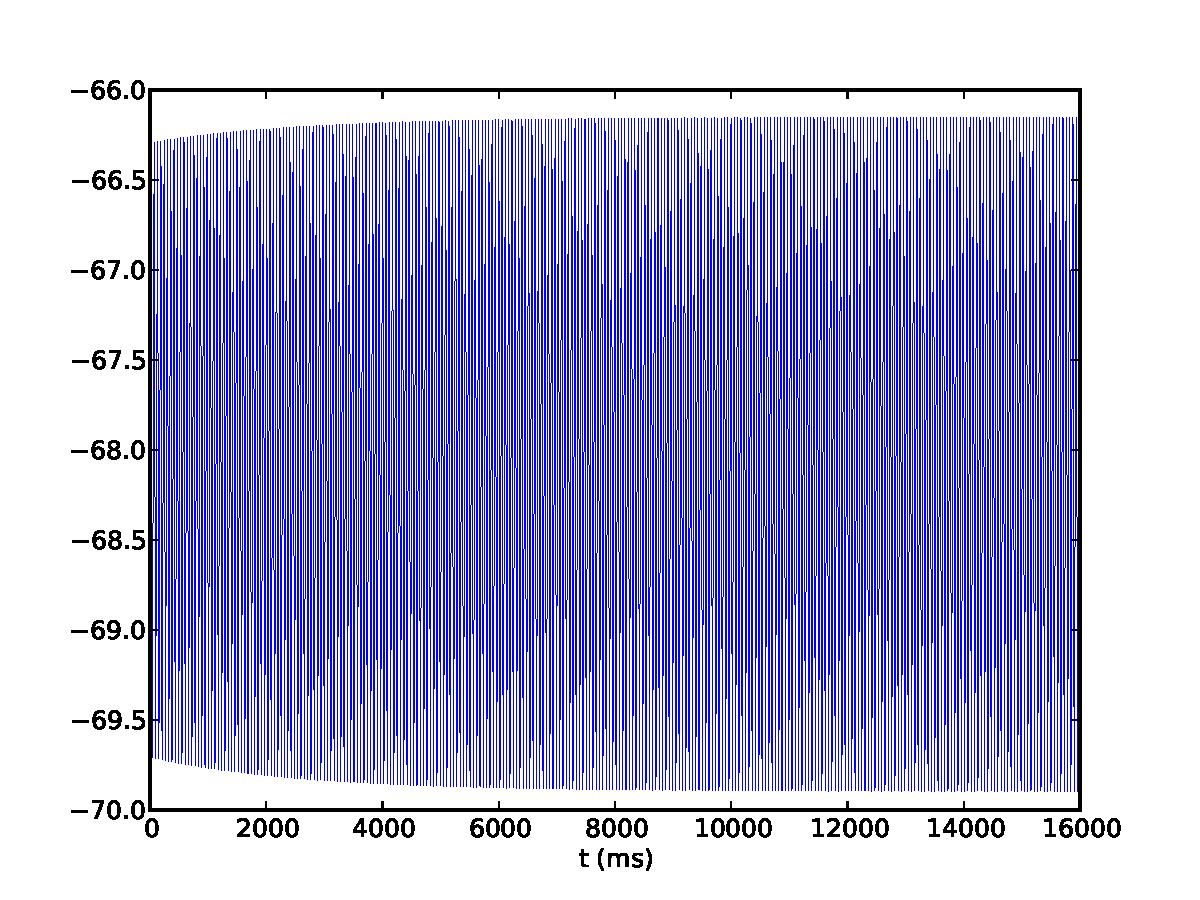
\includegraphics[scale=0.35]{chosen-frontiers-2012/00460-3-he-intra.pdf}
		\label{fig:460_a}
		\caption{$h_e (mV)$}
	\end{subfigure}
	\begin{subfigure}[b]{0.5\textwidth}
		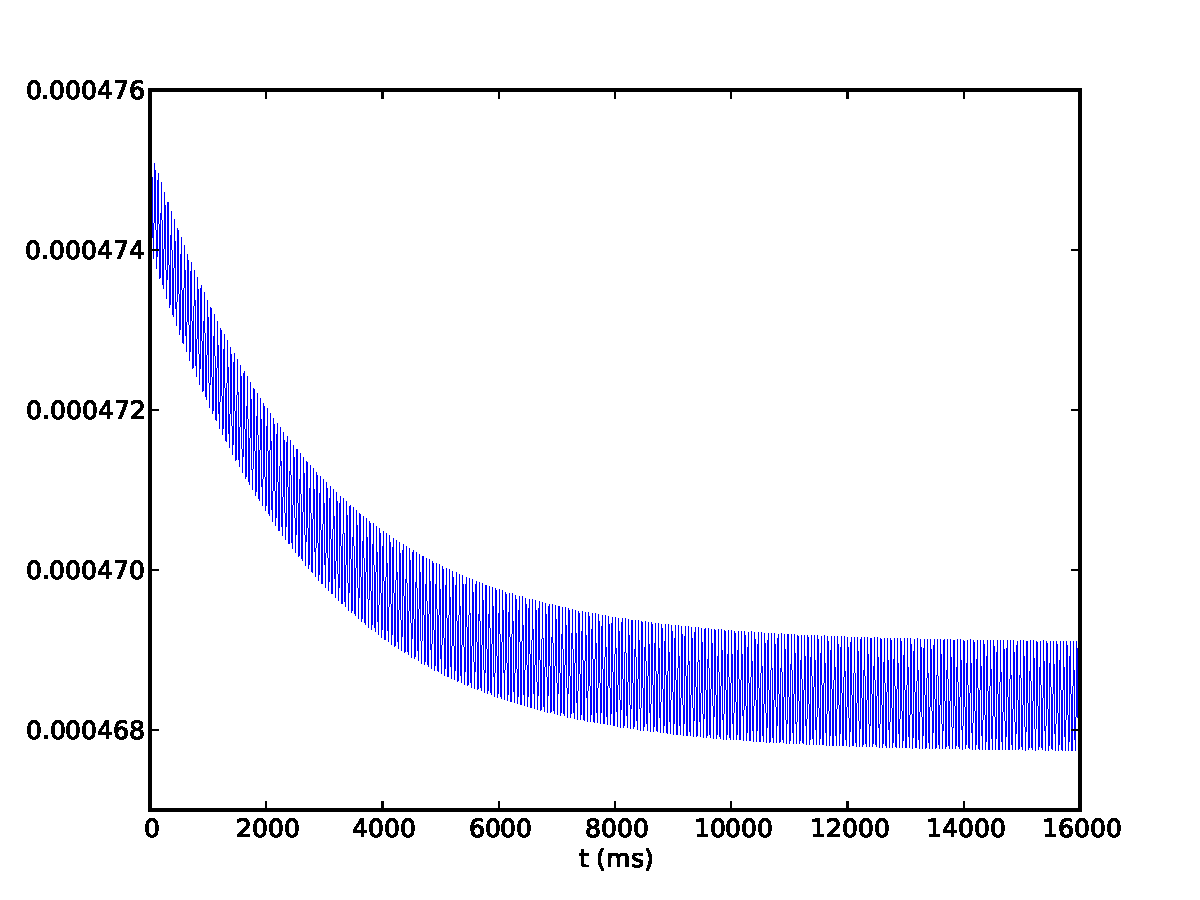
\includegraphics[scale=0.35]{chosen-frontiers-2012/00460-3-slow-intra.pdf}
		\label{fig:460_b}
		\caption{$\zeta_e (UNITS)$}
	\end{subfigure}
	\begin{subfigure}[b]{0.5\textwidth}
		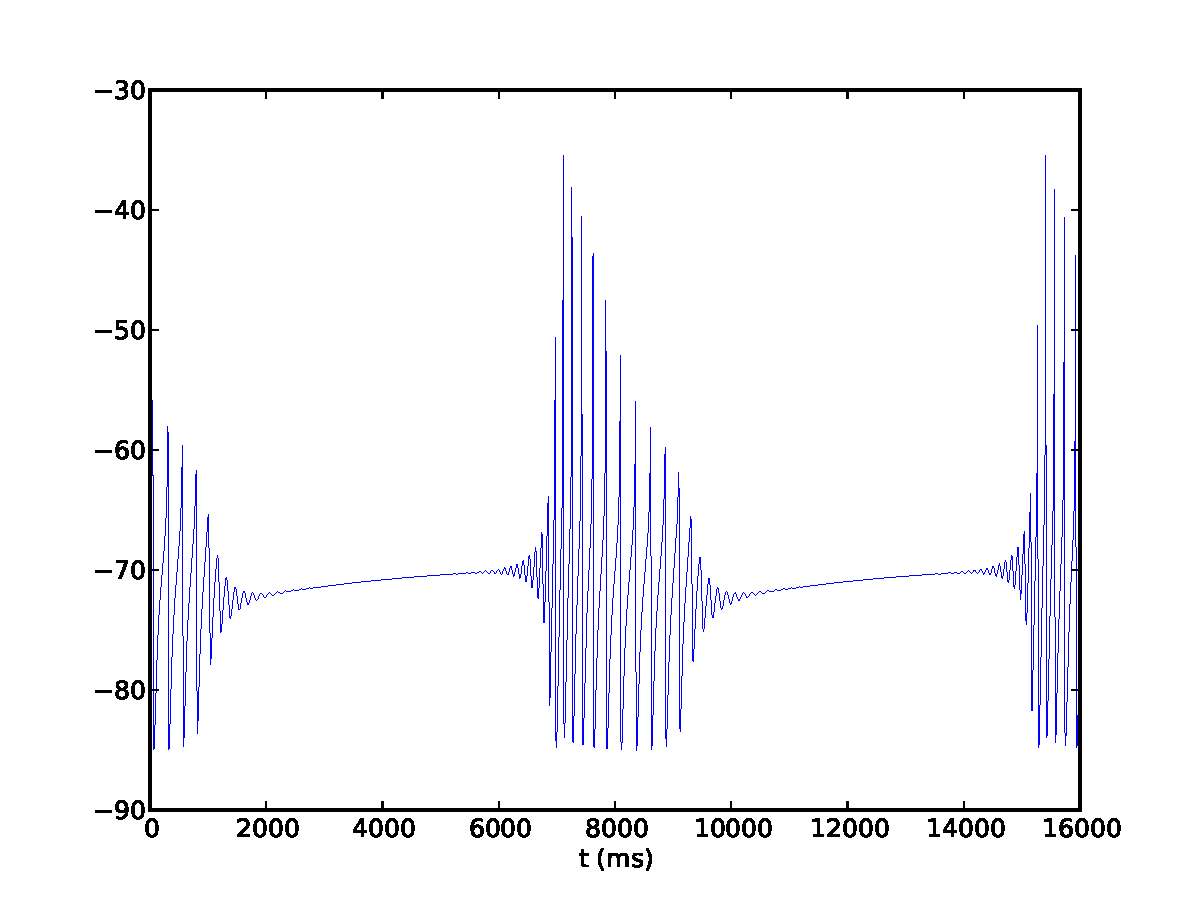
\includegraphics[scale=0.35]{chosen-frontiers-2012/00460-0_7-he-intra.pdf}
		\label{fig:460_c}
		\caption{$h_e (mV)$}
	\end{subfigure}
	\begin{subfigure}[b]{0.5\textwidth}
		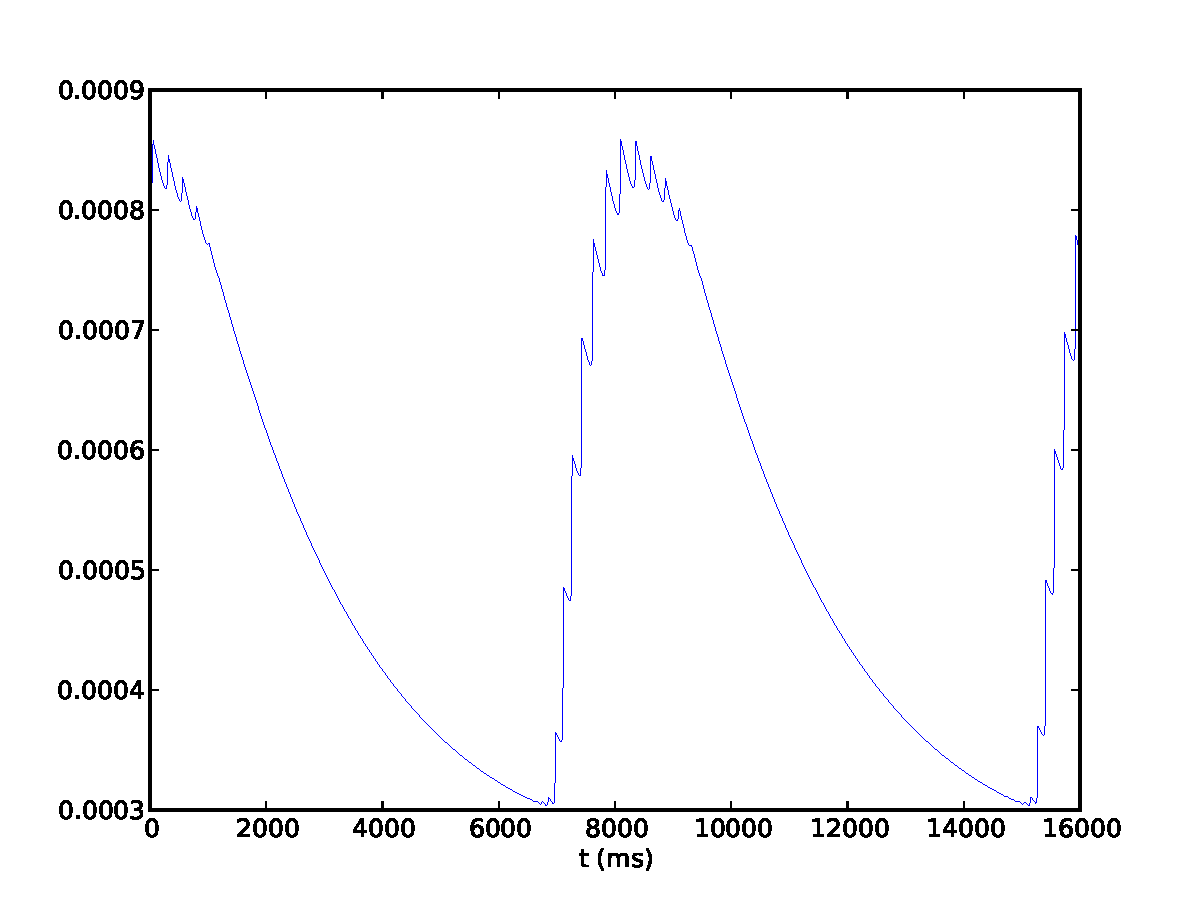
\includegraphics[scale=0.35]{chosen-frontiers-2012/00460-0_7-slow-intra.pdf}
		\label{fig:460_d}
		\caption{$\zeta_e (UNITS)$}
	\end{subfigure}
      \label{fig:emerging_slow_zeta}
	\caption{$h_e$ along with $\zeta_e$ for the model of synaptic/intracellular resource utilisation. 
	Values as follows:
	\ref{fig:460_a} and \ref{fig:460_b}: $\gamma_{ie}=1.1841867$, $\gamma_{ii}=0.09702306$, \ref{fig:460_a} and \ref{fig:460_b}:  $\gamma_{ie}=0.27631023$, $\gamma_{ii}=0.022638713999999997$. 
	All other parameters:
$\Lambda_{ee}: 0.418331295, \Lambda_{ei}: 0.418331295, N^{\alpha}_{ee}: 3524.127975, N^{\alpha}_{ei}: 1178.475832,
N^{\beta}_{ee}: 4567.016139, N^{\beta}_{ei}: 2946.029337, N^{\beta}_{ie}: 705.6645138, N^{\beta}_{ii}: 155.6924316,
\Gamma_{ee}: 1.030206899, \hat{\Gamma_{ei}}: 1.245480131, \hat{\Gamma_{ie}}: 1.661138507, \Gamma_{ii}: 1.144879622,
g_e: 0.7, \gamma_{ee}: 0.71336694981, \gamma_{ei}: 0.53411167, \chi_{ee}: 700.0, \chi_{ei}: 700.0, h^{rest}_e: -79.27217543,
h^{eq}_{ee}: -19.32193417, h^{eq}_{ei}: -8.307573166, h^{rest}_i: -76.08372036, h^{eq}_{ie}: -85.45750982,
h^{eq}_{ii}: -84.48223465, \mu_e: -54.37736285, \mu_i: -54.60726943,
p_{ee}: 6.8330303706, p_{ei}: 9.2679440497,
p_{ie}: 0.0, p_{ii}: 0.0, \phi_{ie}: 0, \phi_{ii}: 0, S^{max}_e: 0.0637001, S^{max}_i: 0.0838227,
\sigma_e: 4.16943943, \sigma_i: 2.126102814, \tau_e: 73.3, \tau_i: 75.2, \tau^{slow}: 3665.0,
  v_{ee}: 0.839055, v_{ei}: 0.839055$
}
\end{figure}

\begin{figure}
	\begin{subfigure}[b]{1\textwidth}
		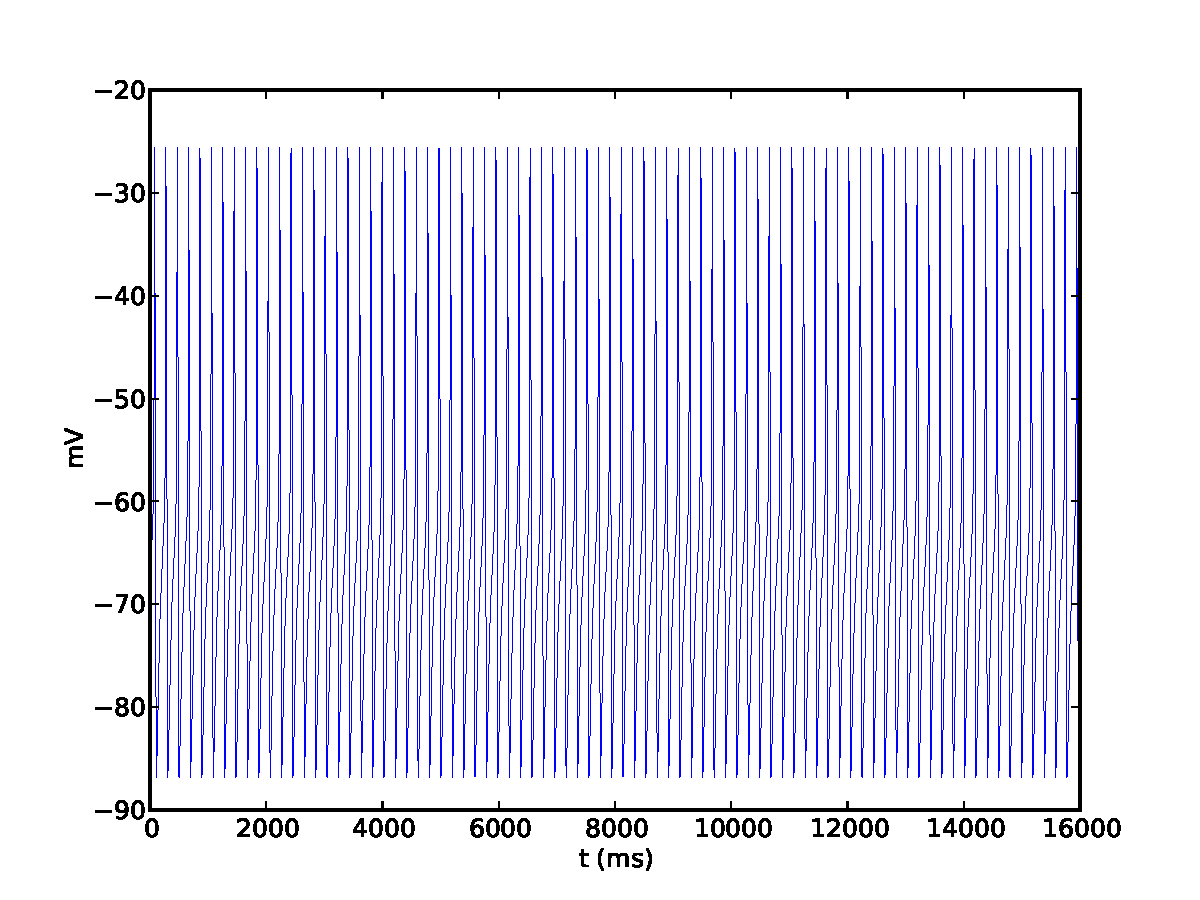
\includegraphics[scale=0.32]{chosen-frontiers-2012/00214-1-0_5-5-0_5-he-phi.pdf}
		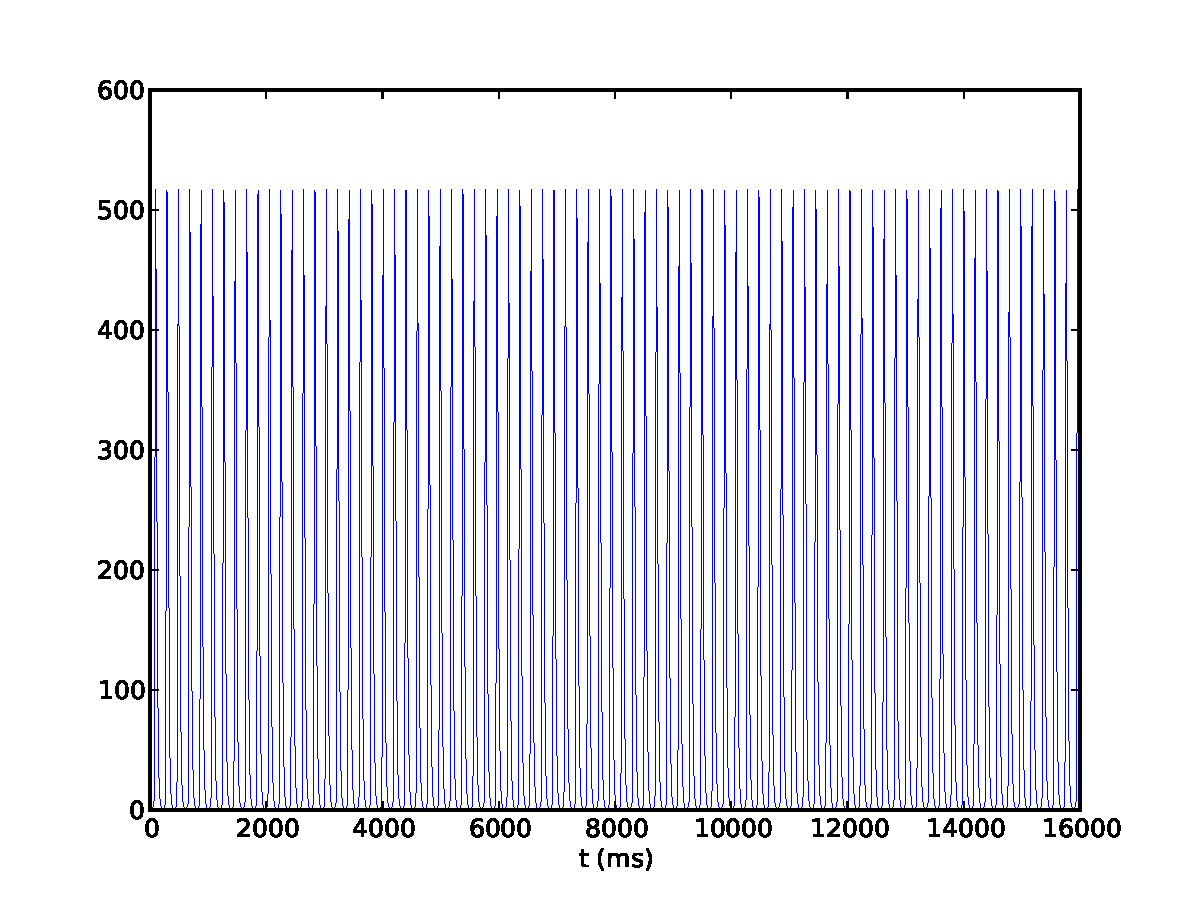
\includegraphics[scale=0.32]{chosen-frontiers-2012/00214-1-0_5-5-0_5-phi_ei-phi}
		\label{fig:214-1-0_5-5-0_5}
		\caption{$h_e (mV)$ and $\phi_{ei}$}
	\end{subfigure}

	\begin{subfigure}[b]{1\textwidth}
		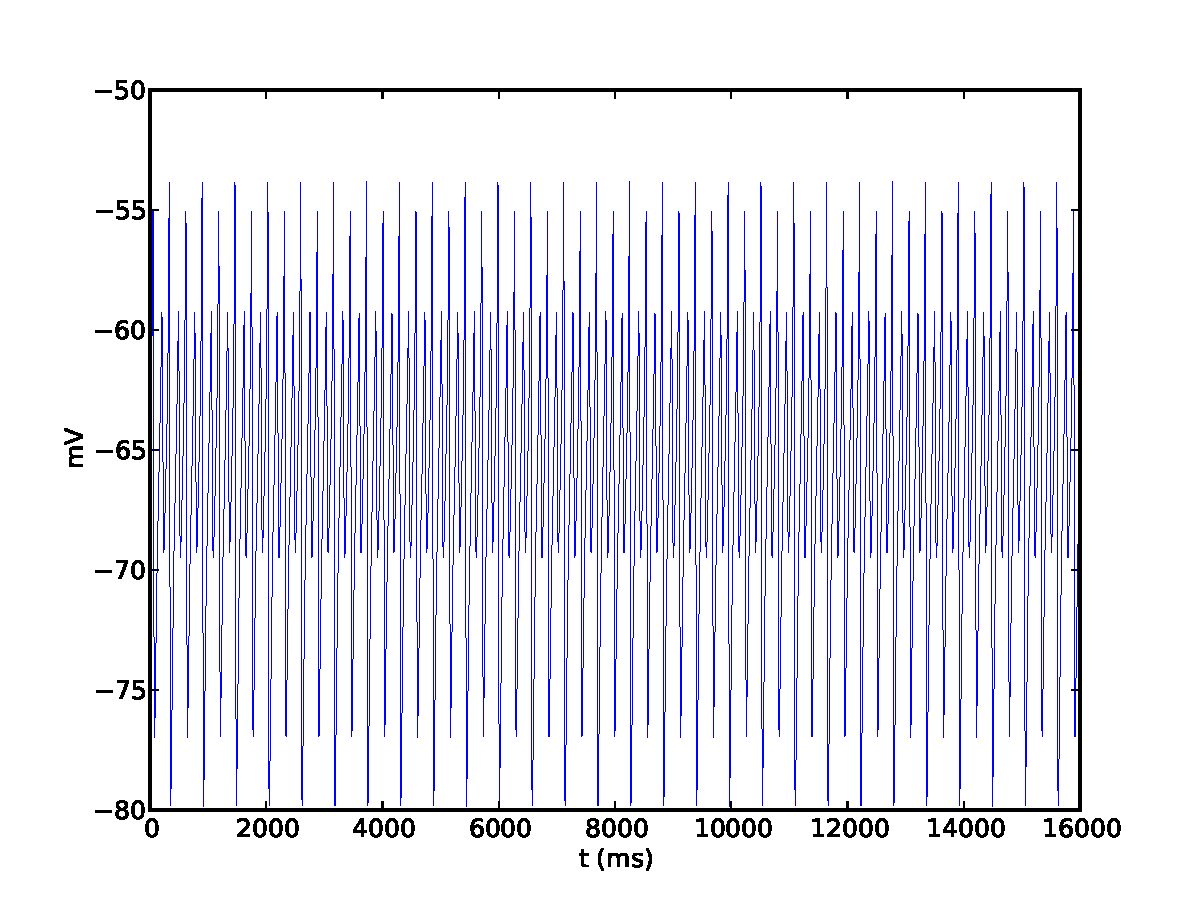
\includegraphics[scale=0.32]{chosen-frontiers-2012/00214-1-0_1-5-0_2-he-phi.pdf}
		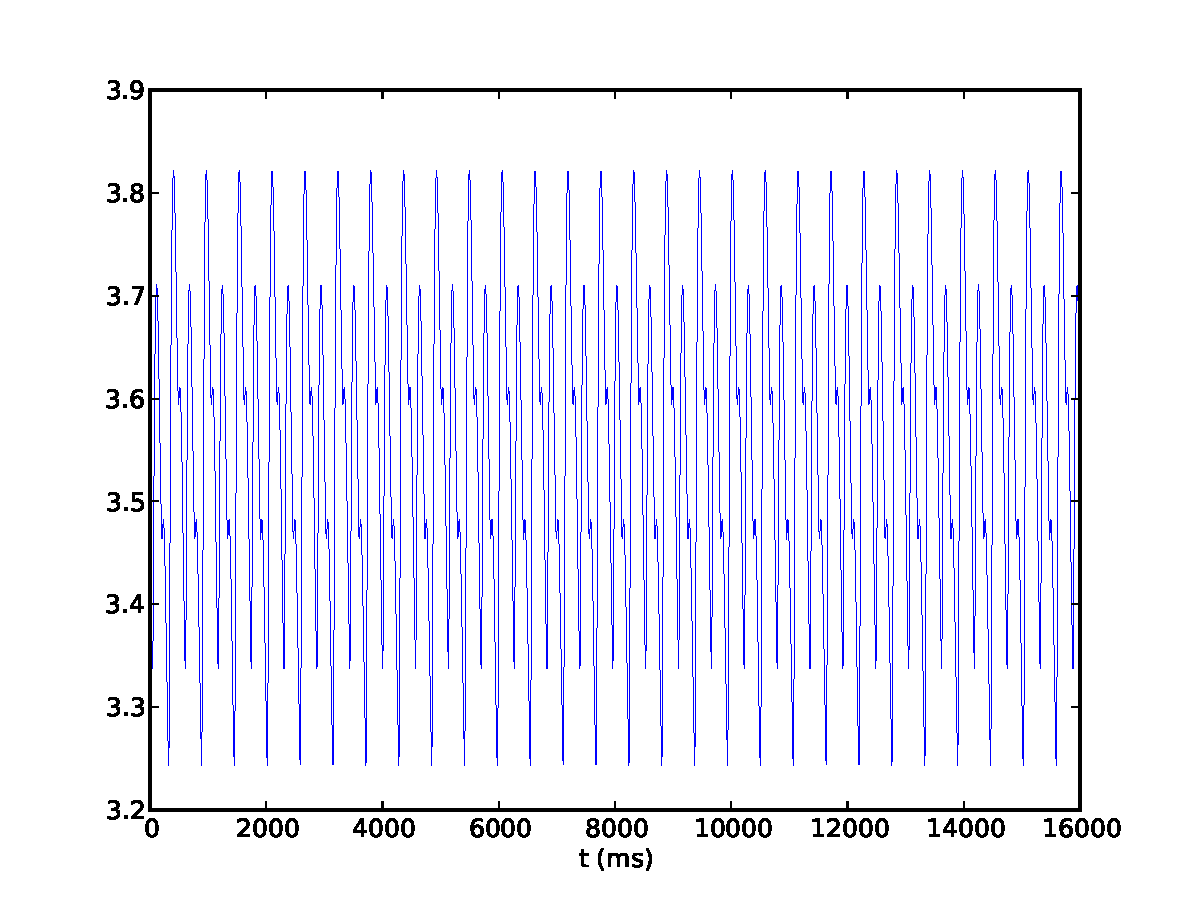
\includegraphics[scale=0.32]{chosen-frontiers-2012/00214-1-0_1-5-0_2-phi_ei-phi}
		\label{fig:214-1-0_1-5-0_2}
		\caption{$h_e (mV)$ and $\phi_{ei}$}
	\end{subfigure}

	\begin{subfigure}[b]{1\textwidth}
		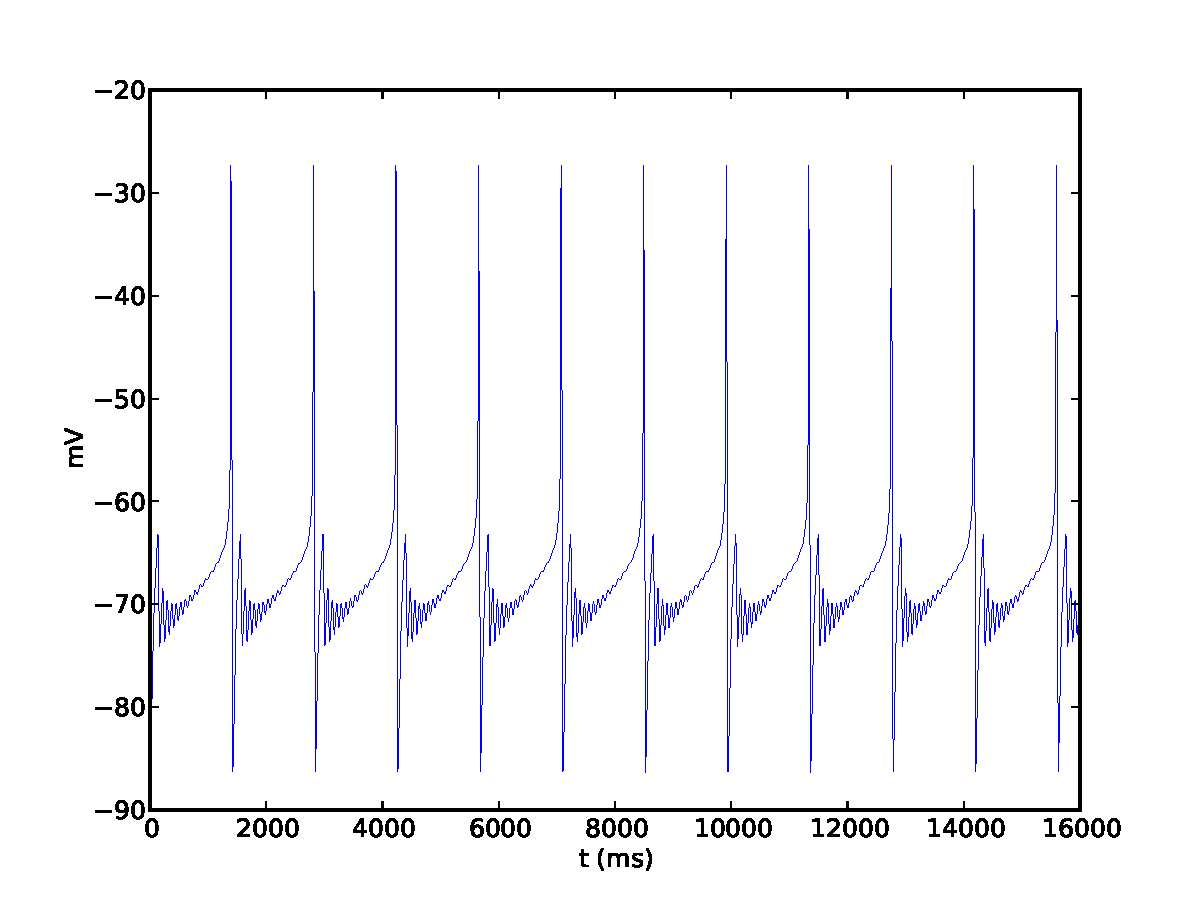
\includegraphics[scale=0.32]{chosen-frontiers-2012/00214-1-0_1-5-0_1-he-phi.pdf}
		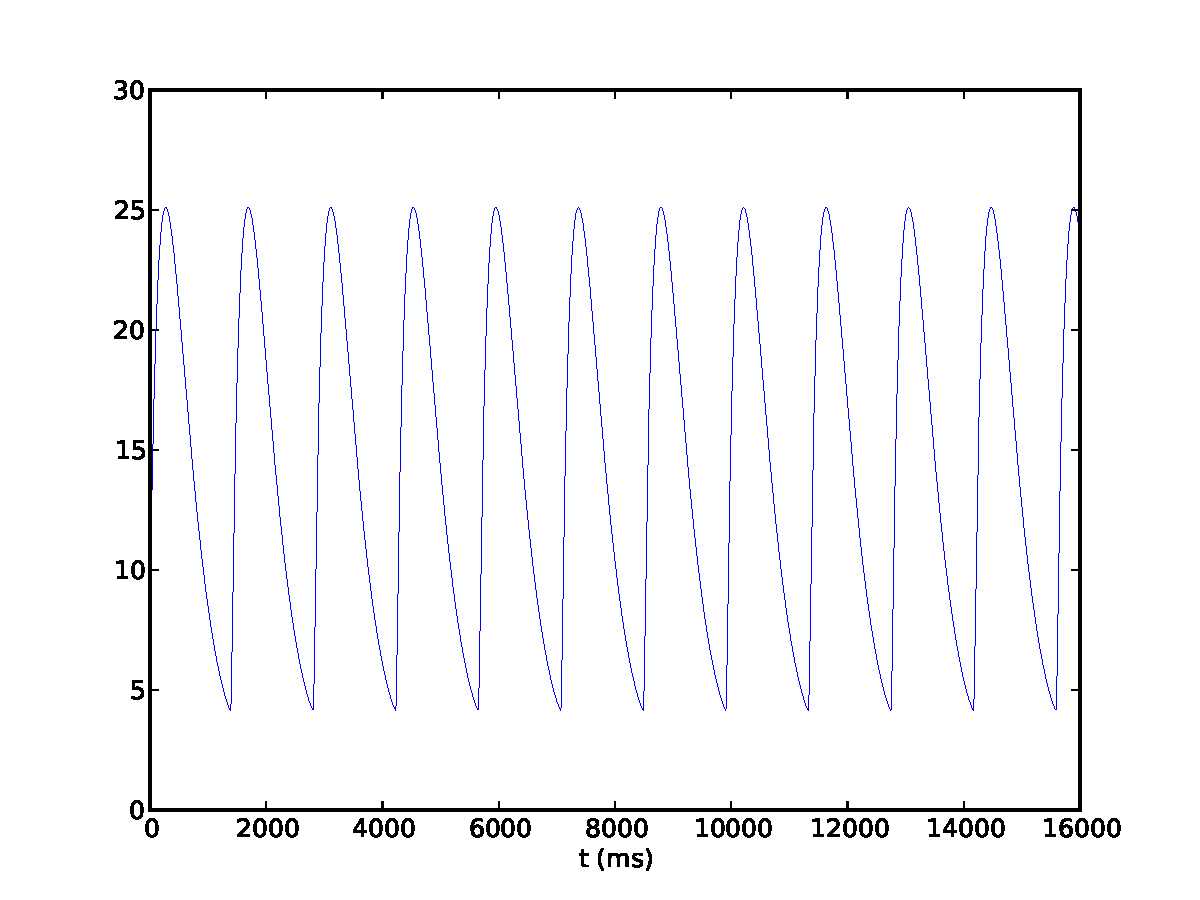
\includegraphics[scale=0.32]{chosen-frontiers-2012/00214-1-0_1-5-0_1-phi_ei-phi}
		\label{fig:214-1-0_1-5-0_2}
		\caption{$h_e (mV)$ and $\phi_{ei}$}
	\end{subfigure}
	\label{fig:phi_dyn}
	\caption{Illustrating the emergence of a slow system ($\phi_{ei}$) as parameters $v_{ei}$ and $\Lambda_{ei}$ are decreased. \\
	Parameter values as follows:\\
	a. $v_{ei} = 0.4122915$ and $\Lambda_{ei} = 0.1943756305$\\
	b. $v_{ei} = 0.0824583$ and $\Lambda_{ei} = 0.0777502522$\\
	c. $v_{ei} = 0.0824583$ and $\Lambda_{ei} = 0.0388751261$\\
All other parameters:\\
$\Lambda_{ee}: 1.943756305, N^{\alpha}_{ee}: 2661.274299, N^{\alpha}_{ei}: 2415.41369,
N^{\beta}_{ee}: 4537.657838, N^{\beta}_{ei}: 4285.318574, N^{\beta}_{ie}: 496.4015214, N^{\beta}_{ii}: 989.8177416,
\Gamma_{ee}: 0.426272815, \Gamma_{ei}: 1.718762667, \Gamma_{ie}: 0.857083964, \Gamma_{ii}: 1.322388202,
\gamma_{ee}: 0.78950312677, \gamma_{ei}: 0.82632296, \gamma_{ie}: 0.14776569,
\gamma_{ii}: 0.04887233, h^{rest}_e: -75.54580909, h^{eq}_{ee}: -16.50733437, h^{eq}_{ei}: -2.729873877,
h^{rest}_i: -75.55674507, h^{eq}_{ie}: -88.67197452, h^{eq}_{ii}: -85.43395694,
\mu_e: -42.50180811, \mu_i: -48.70101116, p_{ee}: 7.1858700524, p_{ei}: 6.7944395893, p_{ie}: 0.0, p_{ii}: 0.0, \phi_{ie}: 0,
\phi_{ii}: 0, S^{max}_e: 0.450176, S^{max}_i: 0.07468, \sigma_e: 5.024823991,
\sigma_i: 3.22531141, \tau_e: 38.9, \tau_i: 137.859, v_{ee}: 0.824583$}
\end{figure}

\begin{figure}
	\begin{subfigure}[b]{0.3\textwidth}
		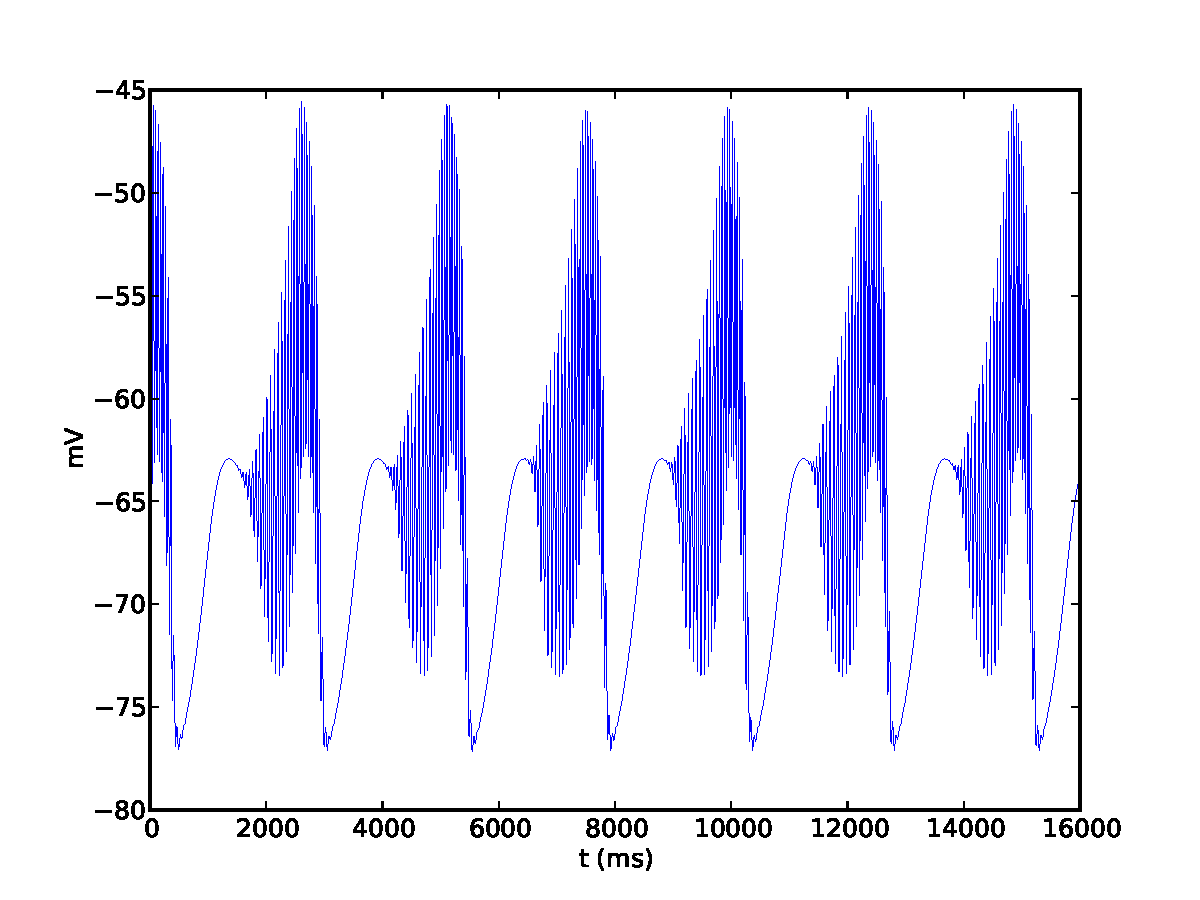
\includegraphics[scale=0.22]{chosen-frontiers-2012/00416-he-phi.pdf}
		\label{fig:416_phi_a}
		\caption{$h_e (mV)$}
	\end{subfigure}
	\begin{subfigure}[b]{0.3\textwidth}
		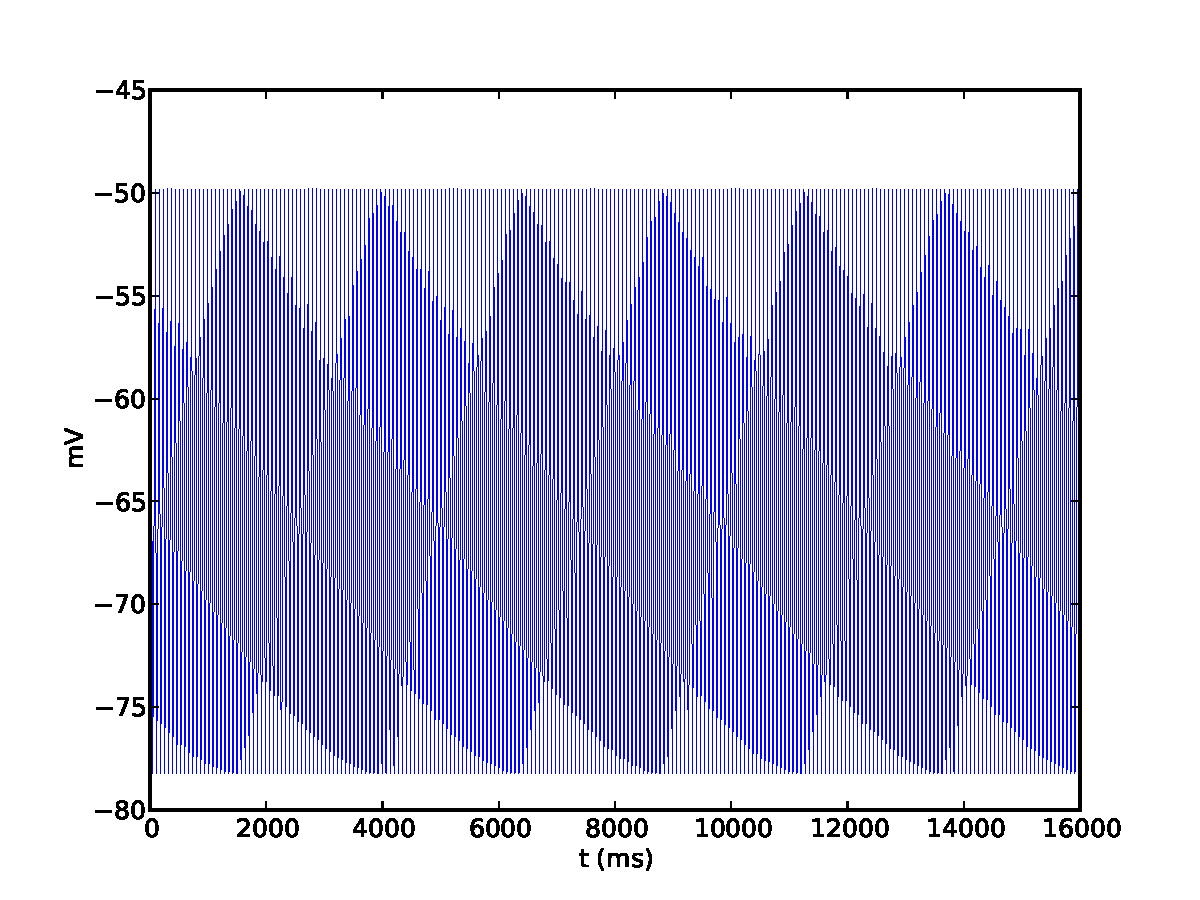
\includegraphics[scale=0.22]{chosen-frontiers-2012/00416-0_5-2-1-he-phi.pdf}
		\label{fig:416_phi_b}
		\caption{$h_e (mV)$}
	\end{subfigure}
	\begin{subfigure}[b]{0.3\textwidth}
		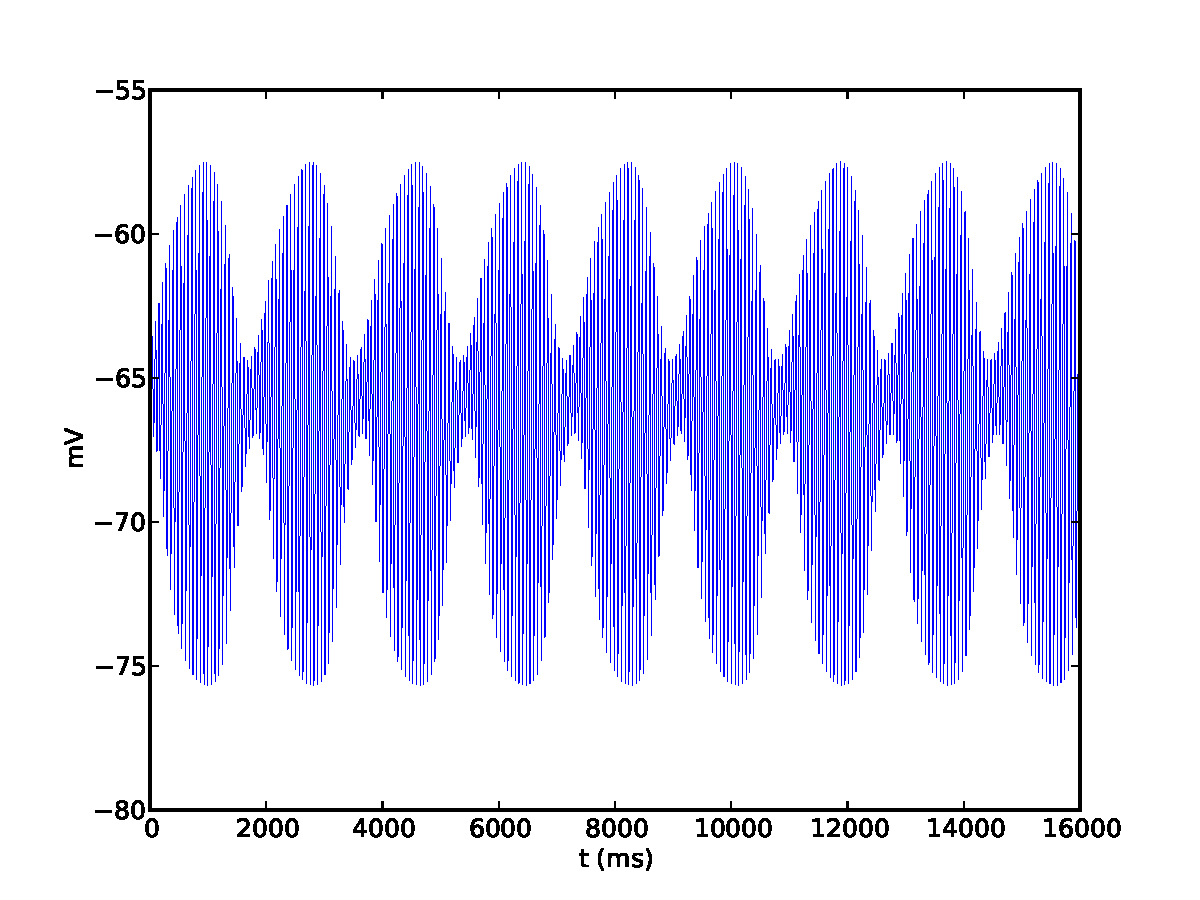
\includegraphics[scale=0.22]{chosen-frontiers-2012/00416-1_1-2-1-he-phi.pdf}
		\label{fig:416_phi_c}
		\caption{$h_e (mV)$}
	\end{subfigure}

	\label{fig:phi_fast_var}
	\caption{Effect of modifying fast system parameters $\gamma_{ie}$, $\gamma_{ii}$, $\Gamma_{ie}$ and $\Gamma_{ii}$ with BS arising from slowing of the long range coupling in the cannonical model of Liley et al.\\
	a. $\Gamma_{ie}: 1.42852881, \Gamma_{ii}: 0.14073783, \gamma_{ie}: 0.45787892, \gamma_{ii}: 0.09011466$ \\
	b. $\Gamma_{ie}: 2.85705762, \Gamma_{ii}: 0.28147566, \gamma_{ie}: 0.22893946,  \gamma_{ii}: 0.04505733$\\
	c. $\Gamma_{ie}: 2.85705762, \Gamma_{ii}: 0.28147566, \gamma_{ie}: 0.503666812,  \gamma_{ii}: 0.099126126$\\
All other parameters:\\
$\Lambda_{ee}: 0.33012064, \Lambda_{ei}: 0.033012064, N^{\alpha}_{ee}: 2342.99410942, N^{\alpha}_{ei}: 2635.01259668,
N^{\beta}_{ee}: 4016.1981429, N^{\beta}_{ei}: 4356.20256437, N^{\beta}_{ie}: 634.73935613, N^{\beta}_{ii}: 473.38388612,
\Gamma_{ee}: 0.13699266, \Gamma_{ei}: 0.4439827, \gamma_{ee}: 0.244953287255, \gamma_{ei}: 0.82969594, h^{rest}_e: -61.7485641, h^{eq}_{ee}: 5.73011624, h^{eq}_{ei}: 2.099135,
h^{rest}_i: -64.46142322, h^{eq}_{ie}: -81.67044311, h^{eq}_{ii}: -82.29433835, \mu_e: -53.10048735, \mu_i: -53.68380602, p_{ee}: 3.6997382629, p_{ei}: 0.60015865013, p_{ie}: 0.0, p_{ii}: 0.0, \phi_{ie}: 0,
\phi_{ii}: 0, S^{max}_e: 0.0930382, S^{max}_i: 0.0648537, \sigma_e: 4.64535035,
\sigma_i: 3.10925431, \tau_e: 86.1876, \tau_i: 65.0391, v_{ee}: 0.160606, v_{ei}: 0.160606$
}

\end{figure}


\section{Discussion}

\subsection{Long range coupling}
Although at this stage there is currently little evidence to suggest anaesthetics slow conduction velocities, it is
widely documented that axonal conduction velocities are significantly decreased in hypothermia. Decreases of up to 5\%
per $^{\circ}{\rm C}$ for conduction velocity have been reported (Waxman 1980) .

As BS has been observed associated with hypothermia(Schwartz et al, 1989; Akrawi et al 1996), we can conclude that  a slow system emerging in the long range coupling via a slowing of axonal conduction velocity is a possible route
to BS.

\subsection{Onset of bursting may emerge from parametric changes in the 'fast' system alone}
A wide variety of bursting dynamics have been observed via simple parametric alteration. It is demonstrated that parametric variations in
'fast' system variables ($\gamma_{ik}, \Gamma_{ik}, \Gamma_{ek}, \tau_i$) alone can instigate BS and vary its dymaics. It is therefore conceivable that BS is triggered either partially or entirely via a parametric variation in the fast system alone.

From this evidence it is conceivable that the slow systems introduced in the models of thalamic averaging and synaptic/intracellular resource utilisation may be largely unaffected by anaesthesia. In this case the triggering of BS would be almost entirely due the the anaesthetic effect on the 'fast' system.

\subsection{Multiple origins for bursting possible}
We have presented results that demonstrate that there are a variety of physiologically plausible mechanisms that bring about
BS. Concordant with experimental evidence(ref), intrinsic and extrinsic cortical mechanisms have been
presented that can produce BS in the model of Liley et al.

The ability to demonstrate BS within the model of Liley et al. through both the introduction of physiologically
plausible slow mechanisms and through parametric changes in the cannonical model, suggests that BS may be a phenomenon that has multiple origins. Further work is needed to investigate the interactions
between the introduced and emergent slow systems.

\subsection{Further investigations}
The current investigations have focussed on the spatially homogeneous case for the model of Liley et al. (i.e. $\nabla^2 =
0$ in \ref{eq:phi}). The cortical phase synchrony(ref?) of burst suppression therefore has not as yet been investigated.

This investigation considered each emergent slow system orthogonally and we have not as yet investigated the
interactions between the presented emergent slow system in a unified model that covers all the presented augmentations to the cannonical model of Liley et al.


\begin{thebibliography}{999}

\bibitem{izikevich2007_1}
  Eugene M. Izhikevich,
  Dynamical Systems in Neuroscience: the geometry of excitability and bursting:329-344,
  1st Edition,
  2010.

\end{thebibliography}

\end{document}

